\documentclass[        
a4paper,          
12pt,             
chapter=TITLE,   
section=Title,    
subsection=Title,
oneside,          
english,          
spanish,          
brazil,           
fleqn            
]{lib/abntex2}
\input{lib/preambulo}
\usepackage{pdfpages}
\usepackage{pgfplots}
\pgfplotsset{compat=1.18}
\usepackage{multirow}
\usepackage{makecell}
\usepackage{pdflscape}
\usepackage{ragged2e}
%\usepackage{acro}
%\usepackage{acro}
\DeclareAcronym{uffs}{
	short=UFFS,
	long=Universidade Federal da Fronteira Sul
}
\DeclareAcronym{ia}{
	short=IA,
	long=Inteligência Artificial
}
\DeclareAcronym{adf}{
	short=ADF,
	long=Dickey-Fuller aumentado
}
\DeclareAcronym{fac}{
	short=FAC,
	long=Função de Autocorrelação
}
\DeclareAcronym{facp}{
	short=FACP,
	long=Função de Autocorrelação Parcial
}
\DeclareAcronym{aic}{
	short=AIC,
	long=Critério de Informação de Akaike
}
\DeclareAcronym{bic}{
	short=BIC,
	long=Critério de Informação Baysiano
}

\DeclareAcronym{fmi}{
	short=FMI,
	long=Fundo Monetário Internacional
}
\DeclareAcronym{ma}{
	short=MA,
	long=Média Móvel
}

\DeclareAcronym{ar}{
	short=AR,
	long=Auto-Regressivo
}
% Configurações do modelo 
\removerbordasdohyperlink{sim}
%\cordohyperlink{nao} 
%\citeoption{abnt-full-initials=yes}

% Comando para citar no padrão ABNT
% Capa

\begin{document}
    \begin{capa}
            \begin{center}
                
\includegraphics[width=2cm]{LOGO_UFFS.png}\\[0.5cm]
                \textbf{UNIVERSIDADE FEDERAL DA FRONTEIRA SUL}\\
                \textbf{CAMPUS LARANJEIRAS DO SUL}\\
                \textbf{CIÊNCIAS ECONÔMICAS}\\[4cm]
                
                \textbf{LEONILSO FANDRES WRUBLAK}\\[4cm]
                
                \textbf{AS MÁQUINAS ECONÔMICAS: PREDIÇÃO DO PIB BRASILEIRO UTILIZANDO INTELIGÊNCIA ARTIFICIAL}\\[7cm]
%                Título provisório
                
                \textbf{LARANJEIRAS DO SUL - PR}\\
                \textbf{2026}
            \end{center}
        \end{capa}
        \setcounter{page}{1}
        \begin{folhaderosto}
            \begin{center}
                \textbf{LEONILSO FANDRES WRUBLAK}\\[4cm]
                
                \textbf{AS MÁQUINAS ECONÔMICAS: PREDIÇÃO DO PIB BRASILEIRO UTILIZANDO INTELIGÊNCIA ARTIFICIAL}\\[3cm]
            \end{center}
            
            \vspace*{\fill}
            \hfill
            \parbox{8cm}{
                Trabalho de Conclusão de Curso apresentado ao Curso de Ciências Econômicas da
                Universidade Federal da Fronteira Sul (UFFS), como requisito para obtenção do
                título de Bacharel em Ciências Econômicas.}
            
            \vspace*{2cm}
            
            \begin{center}
                Orientador: Prof. Dr. Alexandre Manoel dos Santos (UFFS)\\[2cm]
                LARANJEIRAS DO SUL - PR\\
                2026
            \end{center}
        \end{folhaderosto}
        
        % Comandos para incluir ficha e folha após aprovação 
        % \includepdf[pages=1]{}
        % \includepdf[pages=1, fitpaper=true]{}

        % --- Modelo para Folha de Aprovação ---
        \begin{folhadeaprovacao}
            
            \begin{center}
                {\textbf{LEONILSO FANDRES WRUBLAK}}
                
                \vspace*{2cm}
                
                {\textbf{AS MÁQUINAS ECONÔMICAS:}}\\
                \vspace{0.5cm}
                {PREDIÇÃO DO PIB BRASILEIRO UTILIZANDO INTELIGÊNCIA ARTIFICIAL}
            \end{center}
            
            \vspace{2cm}
            
            \hfill
            \parbox{8cm}{
                Trabalho de Conclusão de Curso apresentado ao Curso de Ciências Econômicas da
                Universidade Federal da Fronteira Sul (UFFS), como requisito para obtenção do
                título de Bacharel em Ciências Econômicas.}
            
            \vspace{1.5cm}
            
            \noindent
            \begin{center}
                        Este trabalho foi defendido e aprovado pela banca em DD/MM/AAAA.
            \end{center}
                    
            \vspace{2cm}
            
            \begin{center}
                BANCA EXAMINADORA
            \end{center}
            
            \vspace{1.5cm}
            
            \noindent
            \begin{center}
                \begin{tabular}{c}
                    \rule{10cm}{0.4pt}\\
                    Prof. Dr. Alexandre Manoel dos Santos - UFFS\\
                    Orientador
                \end{tabular}
            \end{center}
            
            \vspace{1.5cm}
            
            \noindent
            \begin{center}
                \begin{tabular}{c}
                    \rule{10cm}{0.4pt}\\
                    Professor(a) 1\\
                    Avaliador
                \end{tabular}
            \end{center}
            
            \vspace{1.5cm}
            
            \noindent
            \begin{center}
                \begin{tabular}{c}
                    \rule{10cm}{0.4pt}\\
                    Professor(a) 2\\
                    Avaliador
                \end{tabular}
            \end{center}
            
        \end{folhadeaprovacao}

    % imprimir dedicatória e agradecimentos funcionam bem com a norma da universidade
    \imprimirdedicatoria{1-pre-textuais/dedicatoria}
	\imprimiragradecimentos{1-pre-textuais/agradecimentos}

    % O epigrafo fica bugado com o modelo portanto estou usando formatação manual

    \begin{epigrafe} 
	    \vspace*{\fill}
        \begin{flushright}
            \parbox{0.6\textwidth}{ 
                \vspace*{\fill}
\begin{flushright}
	\parbox{0.5\textwidth}{ 
		"De fato, sabemos muito pouco sobre o futuro. A base real para formar expectativas sobre o rendimento futuro de um investimento é extremamente frágil. Nossas decisões de investimento [...] dependem de um estado de confiança. Muitas vezes, sabemos que não sabemos; mas mesmo assim temos que agir." 
	}
	
	\vspace{0.5cm} % Adiciona um pequeno espaço entre a citação e o autor
	
	\citem[p. 161]{KEYNES1936}
\end{flushright} 
            }
        \end{flushright}
	\end{epigrafe}

    % Resumo e Abstract
    \imprimirresumo{1-pre-textuais/resumo}
	\imprimirabstract{1-pre-textuais/abstract}

    % Listas
    \newpage
	\listoffigures*
	\newpage
	\listoftables*
	\newpage
	\printacronyms[name={LISTA DE SIGLAS}] % Nome modificado para a formatação da UFFS
	\newpage

    \tableofcontents*

    \newpage
	\textual
    \chapter{Introdução}
\label{cap:introducao}

	Para onde vamos? uma das questões fundamentais da natureza humana, estudada pelas mais diferentes ciências, desde exatas às sociais. Dentre as ciências que buscam a resposta do para onde iremos, temos a economia, uma ciência que encontra-se no meio termo, a chamada social aplicada. Inicialmente pode parecer estranho, mas boa parte do trabalho de um economista é entender os fatos passados e presentes para predizer (ou tentar) o  futuro, mas a pergunta que fica é por quê a economia se preocupa tanto com o futuro?

Para \citeonline[p. 1]{mankiw2025introduccao} "a economia é o estudo de como a sociedade administra seus recursos escassos", é essa escassez \footnote{escassez:  natureza limitada dos recursos da sociedade \citem[p. 1]{mankiw2025introduccao}} que é o motivador para a preocupação com o futuro, afinal se tivéssemos recursos ilimitados não haveria motivo para estudar economia. Mas este não é o caso, existe limitação de recursos, e devemos saber qual é a melhor maneira de alocar esses recursos.

Para um melhor enfoque, a economia se subdivide em duas grandes áreas, a microeconomia, voltada para o estudo da firma (empresas), e a macroeconomia, que estuda os agregados econômicos \citem{Vasconcelos}

No presente trabalho nos voltaremos para a macroeconomia, área da economia que surge no inicio do século XX, devido as intensas mudanças sociais, políticas e econômicas que ocorreram no período, a principal obra referência da macroeconomia é o livro de John Maynard Keynes: \textit{Teoria Geral do Emprego, do Juro e da Moeda} \citeyear{KEYNES1936}, onde o autor traz os principais fundamentos da macroeconomia que é estudada hoje na academia e executada nos governos.


Um desses conceitos fundamentais que Keynes aborda é a noção de incerteza
\begin{citacao}
	De fato, sabemos muito pouco sobre o futuro. A base real para formar expectativas sobre o rendimento futuro de um investimento é extremamente frágil. Nossas decisões de investimento [...] dependem de um estado de confiança. Muitas vezes, sabemos que não sabemos; mas mesmo assim temos que agir. \citem[p. 161]{KEYNES1936}
\end{citacao}
Com essa noção de incerteza definida por Keynes podemos relacionar com aquela nossa questão fundamental, gestores mundiais, sejam eles públicos ou privados, buscam maneiras de observar dados históricos e com um certo intervalo de confiança tentar "prever o futuro", para justamente, combater a incerteza.


A incerteza 
%	traz desconfiança, e a desconfiança, por sua vez, 
gera perguntas, e encontrar as respostas para essas perguntas vai muito além da impressão pessoal
%	\textit{feeling}
%	\footnote{\textit{feeling}: impressão, sentimento, pressentimento}
do gestor. Os gestores precisam de informação para suas decisões, e para \citeonline{laudon2022sistemas} os sistemas de informação são essenciais para alcançar objetivos estratégicos dos negócios. Na era digital, o grande volume de dados gerados pelos sistemas de informação podem ser usados como fontes, praticamente inesgotáveis de dados.

Esses grandes volumes de dados, gerados pelos sistemas de informação, são chamados de \textit{big data}. Para \citem[p. 9]{vasconcelos2017poder}  "O \textit{big data} caracterizado por grandes bases de dados com um número elevado de preditores relativos às observações disponíveis". Contudo, somente ter os dados não é o suficiente, e converter esse grande volume de dados em informações não é uma tarefa simples, e exige técnicas sofisticadas de coleta, tratamento e modelagem. Os processos de coleta e tratamento, apesar de fundamentais, serão usados somente como passos anteriores ao da modelagem, que é o enfoque  desse texto.  

% gostaria de trazer um autor sobre modelos econometricos, porém fiquei indeciso













%	Nesse processo a estatística e a ciência de dados trazem o aporte teórico para o tratamento, coleta e transformação desses dados em informações uteis. 


%	Adicioanar a definição de IA, Machine Learning na Introdução não esquecer


\section{Problema de pesquisa}

Avaliar modelos na previsão de variáveis econômicas não é um processo novo, muitos autores já usaram diversas vezes esses modelos.

Em sua dissertação, \citeonline{azevedo2020modelagem} usou o modelo modelo de vetores auto-regressivos (VAR) para análise de séries temporais com variáveis macroeconômicas.
Já \citeonline{fialho2024incerteza} usaram o VAR para entender a dinâmica entre 
incerteza, spread bancário, crédito, consumo, rendimento e taxa de desocupação. 

\citeonline{ciquini2023modelo} avaliou o uso do modelo auto-regressivo de médias móveis (do inglês \textit{AutoRegressive Integrated Moving Average} - ARIMA) para tomada de decisões econômicas. Agora \citeonline{Silva_Clericuzi_Carvalho_2025} apoiaram-se no ARIMA para a predição do PIB brasileiro. 

\citeonline{alves2009nucleo} em sua dissertação de mestrado abordou modelos de fatores dinâmicos (do inglês  \textit{Dynamic Factor Models} - DFM) para entender o núcleo da inflação brasileira. Por outro lado \citeonline{moura2020fragilidade} avaliou os ciclos econômicos brasileiros usando uma combinação entre o DFM e o VAR.

\citeonline{castelli2022modelo} abordou o uso do modelo de amostragem de dados mistos (do inglês \textit{Mixed Data Sampling} - MIDAS) para predizer o PIB com a pesquisa industrial mensal. Assim como \citeonline{micheletti2024avaliaccao} usou modelos de \textit{ensemble stacking} \footnote{\textit{ensemble stacking}: modelos combinados} (dentre eles o MIDAS) para prever o PIB.

A maioria desses autores trabalharam com o que se chamam modelos tradicionais de predição, esses modelos se baseiam em variáveis e proposições bem definidas, o que pode não ser o caso na era do \textit{big data}. Nesse contexto, em que os modelos tradicionais encontram-se limitados, que a inovação surge, nesse caso o uso de técnicas de IA para modelar variáveis econômicas.

Diante do disso a presente pesquisa tende a seguir os passos de \citeonline{kava2022alem} e de \citeonline{rebelo2022interpretabilidade} que comparam, em suas dissertações, modelos de IA com os chamados modelos tradicionais. Contudo, a nossa pesquisa se diferencia dos trabalhos produzidos por testar outros modelos e focar especificamente no PIB brasileiro, para isso norteia-se pela seguinte pergunta: Em que medida modelos preditivos baseados em \ac{ia}, comparados aos modelos tradicionais VAR, ARIMA, DFM e MIDAS, conseguem estimar o PIB brasileiro?

%Como desenvolver um modelo preditivo baseado em IA para efetivamente estimar i]o PIB brasileiro, considerando as diferenças e semlhanças significativas entre os modelos tradicionais VAR, ARIMA, DFM e MIDAS.

\section{Objetivos}
\subsection{Objetivo Geral}
Analisar em que medida modelos preditivos baseados em \ac{ia}, comparados aos modelos tradicionais VAR, ARIMA, DFM e MIDAS, conseguem estimar o PIB brasileiro.

\subsection{Objetivos Específicos}
\begin{itemize}
	\item[a)] Caracterizar os modelos econométricos tradicionais (VAR, ARIMA, DFM e MIDAS) e de IA para a predição do PIB;
	\item[b)] Identificar as diferentes variáveis determinantes na estimativa do PIB;
	\item[c)] Desenvolver um ciclo de vida para a produção de um novo modelo econométrico de IA para a predição do PIB; 
	\item[d)] Comparar o desempenho dos modelos de IA e econométricos tradicionais usando diferentes métricas, como desempenho computacional, precisão e interpretabilidade.
\end{itemize}



\section{Justificativa} 
O presente trabalho justifica-se empiricamente, pois permite que gestores, sejam eles públicos ou privados, utilizem-se de ferramentas estatísticas para tomarem decisões fundamentadas. "A  tomada  de  decisões  empresariais  é  uma  tarefa  complexa  e  fundamental  para  a  sobrevivência de uma organização" \citem[p. 3]{santana2023aprimorando}.

Portanto, a tomada de decisões pode ser fundamentada através dos modelos. Os modelos, mesmo que sejam uma simplificação da realidade, podem aumentar a confiança dos agentes. Segundo \citeonline{KEYNES1936}, essa confiança é um fator que afeta as decisões de investimento.

Já contribuição teórica desse trabalho está alinhada com a avaliação dos diferentes modelos estatísticos para a predição econômica, além é claro, de explorar as novas fronteiras da ciência, com a avaliação de modelos inovadores como os que usam a IA. 


O presente trabalho busca mesclar diferentes modelos, ranqueando seu desempenho, e possibilitando a identificação dos modelos mais adequados para previsão econômica. Para isso é necessário a avaliação métricas estatísticas comuns, semelhante ao que \citeonline{castelli2022modelo} fez, ao comparar modelos de IA com modelos tradicionais, aplicando métricas como coeficiente de determinação ($R^2$), Erro Médio Absoluto (MAE), Erro Quadrático Médio (MSE) para classificar os modelos.

	

    \chapter{Revisão de Literatura}
\label{cap:revisao-literatura}

A presente sessão busca avaliar os estudos até então construídos que perpassam sobre as temáticas correlatas, a evolução dos modelos preditivos, a variável estudada: o \ac{pib}, o uso de modelos preditivos em variáveis macroeconômicas, por fim a avaliação e comparação de modelos preditivos.

Dado esse contexto, a presente revisão de literatura se estruturará da seguinte forma, primeiramente iremos tratar sobre predição econômica de um modo geral e seus principais autores, logo em seguida discutiremos sobre nossa variável foco o \ac{pib}, posteriormente classificaremos os modelos em tradicionais e não-tradicionais, onde será descrito cada modelo o conceito, o histórico, o modelo matemático e a aplicação do mesmo no contexto de predição do \ac{pib}. Após essa conceituação será analisado as métricas de comparação dos modelos, e como elas vem sendo aplicadas. Após a conceituação e análise das métricas de avaliação, serão abordados os trabalhos acadêmicos que já compararam modelos tradicionais e não tradicionais. 

%\section{Estudos Anteriores}
\section{Predição Econômica: O PIB}

% BC CVM FEBRABAM


A predição de variáveis econômicas não é uma tarefa nova, na realidade  estipular o comportamento de variáveis econômicas ao decorrer do tempo é um desejo dos economistas desde o início do século XX. Em seu artigo,  \citeonline{FrischSTATIKKOD} \footnote{Frisch é considerado um dos fundadores da econometria moderna, é a ele atribuído a formulação do termo econometria} trata do conceito da teoria dinâmica, que se subdivide em analítica e histórica, a primeira lida com as leis que regem as flutuações das variáveis, já a segunda trata de aplicar as leis para descrever/prever as variáveis. Essa conceituação teórica de \citeonline{FrischSTATIKKOD} é justamente o que hoje é considerado como econometria, e foi a base para os futuros modelos econométricos e suas aplicações.

Contudo, a economia ficou mais complexa desde 1929, conforme \citeonline{almeida_2001} a economia do início século XX passou por sua fase madura de industrialização incorporou uma grande quantidade de inovações tecnológicas advindos da Segunda Revolução Industrial. Ainda segundo o autor, "a estrutura da produção foi radicalmente transformada pelas mudanças introduzidas nos padrões de trabalho (especialização) e pelos avanços tecnológicos, que aumentaram dramaticamente o produto per capita."\citem[p. 2]{almeida_2001}.

Esse processo se repetiu durante a Terceira Revolução Industrial, \citeonline{junior_2017} aponta que esse processo não foi hegemônico, mas foi  caracterizado por uma revolução  tecno-científica,  não só nas fábricas como na maioria das atividades sócio-econômicas. Durante esse período houve intensas mudanças na atividade produtiva. Contudo alguns autores apontam que a humanidade passou por mais uma revolução, a Quarta Revolução Industrial, ou também chamada de Indústria 4.0.
% Citar autor que confirma a complexidade da economia

O termo industria 4.0\footnote{ Industria 4.0: é a transformação digital na indústria, onde a mesma integra tecnologias como a própria Inteligência Artificial  } é citado pela primeira vez na feira de Hannover como uma nova política Alemã para industrialização \citem{kagermann2013recommendations}. Um dos autores defensores de uma nova fase da industria é \citeonline{martins2021industria}, onde ele argumenta que a Indústria 4.0 traz muitas mudanças no contexto onde ela é aplicada, como novos modelos de negócio e mercados cada vez mais exigentes.

Mas não somente a economia ficou mais complexa, o advento da indústria 4.0  
% Trazer algum autor sobre a industria 4.0
trouxe a possibilidade de coletar e processar grandes volumes de dados através do que chamamos de sistemas de informação. Que para \citeonline{laudon2022sistemas} são essenciais para alcançar objetivos estratégicos dos negócios. 
%	Na era digital, o grande volume de dados gerados pelos sistemas de informação pode ser usada como uma fonte, praticamente inesgotável de informações para tomadas de decisões. 

\begin{citacao}
	A eficácia das políticas depende do uso de todas as informações disponíveis em qualquer momento, incluindo informações prospectivas, como desempenho do mercado de ações e a incerteza da política econômica, disponíveis no ponto de estimativa. \citem[p. 19]{ghosh2023machine}
\end{citacao}

Nesse sentido da importância das informações, muitos indicadores econômicos foram criados, melhorados ou superados, tanto no sentido microeconômico dentro das firmas, assim como indicadores macroeconômicos de grandes agregados. E um desses indicadores macroeconômicos que evoluiu com o tempo busca estimar a produção total interna de uma localidade, o chamado \ac{pib}. Segundo o \ac{ibge} "o \ac{pib} é a soma de todos os bens e serviços finais produzidos por um país, estado ou cidade, geralmente em um ano." \citem[p. 1]{ibge_pib}.

O Banco Central do Brasil trás dois conceitos para o \ac{pib}: "a preços de mercado, (o \ac{pib}) mede o total de bens e serviços produzidos pelas unidades produtoras residentes destinados ao consumo final (exclui o consumo intermediário)." \citem[p. 1]{BCB_SGS_1207}. Além disso o Banco Central do Brasil trás também a ideia do PIB em reais correntes que se refere ao valor dos bens e serviços finais produzidos em determinado período e valorados a preços de mercado do respectivo período, ou seja sem retirar a inflação  \citem{BCB_SGS_1207}. Ambos representam a totalidade de bens e serviços produzidos, e tem o mesmo quantitativo quando analisados no mesmo ano base, mas quando se análisa em períodos de tempo diferentes o PIB a preços de mercado é considerado o PIB real, pois exige um calculo para retirar a inflação das medições do \ac{pib}, enquanto o \ac{pib} em reais correntes sempre se refere ao valor nominal do PIB naquela data, esse geralmente é o valor divulgado pelas bases de dados, como o próprio Banco Central ou o \ac{ibge}.

O conceito internacional de PIB é semelhante com os conceitos do Banco Central do Brasil e do \ac{ibge}. Segundo o \citeonline{BEA_GDP} o PIB mede o valor dos bens e serviços finais produzidos, sem contar os bens e serviços intermediários. A agência estadunidense de divulgação e análise econômica também trás o motivo pelo qual o \ac{pib} é tão importante afinal  "as mudanças no PIB são o indicador mais popular da saúde econômica geral do país" \citem[p. 1]{BEA_GDP}

% Professor adicionei o conceito do IBGE, do Banco Central e do BEA dos EUA

Nesse sentido o \ac{pib} funciona como um termômetro da atividade econômica, e se indicadores refletem a realidade, é lógico pensar que conforme a economia fica complexa, seus indicadores as acompanham, assim como as tentativas de tentar prever seu comportamento.

% Colocar mais complexidade na definição do PIB

E a predição do PIB é algo que é estudado por diversos pesquisadores, muitos dos quais veremos no decorrer dessa revisão de literatura, mas também de órgãos e instituições públicas e privadas, como é o caso do \ac{ipea} que pontua a importância da predição do PIB "para a definição dos parâmetros para o planejamento fiscal e orçamentário do setor público, bem como para a formação de expectativas no setor privado." \citem[p. 6]{santos2022previsao}.

Dado toda essa evolução, é natural perceber a complexificação desse indicador, e fenômenos complexos implicam que métodos tradicionais de predição podem não conseguir descrever a realidade com a mesma precisão da época da qual foram elaborados.

Deste modo, chegamos a um momento de inflexão. Complexidade sistêmica combinada ao grande volume de dados pode fazer com que modelos econométricos tradicionais\footnote{No presente trabalho trataremos que os modelos econométricos tradicionais são aqueles baseados na linearidade das variáveis, ausência de multicolinearidade, homocedasticidade e normalidade dos resíduos} 
%	Traz um autor sobre modelos tradicionais 
não consigam representar a realidade, pois, até que ponto uma simplificação pode representar realmente o comportamento econômico.

Dessa forma, se o tradicional não tem o comportamento esperado recorre-se ao inovador.
%	, conforme .
%	Cabe um Shumpeter aqui
Essa inovação, no contexto dos modelos econométricos, vem através da incorporação de modelos estatísticos que suportam a complexidade econômica, além de tecnologias computacionais que conseguem tratar esse volume de dados gerados pelos sistemas de informação.





\section{Modelos preditivos}

Antes de partirmos para inovação devemos entender o que de fato são esses modelos preditivos. Tomando como princípio o texto de \citeonline{FrischSTATIKKOD} a econometria surge justamente para aplicar as leis que regem a economia, a teoria dinâmica histórica, busca evidenciar as relações entre as variáveis, não por suposição cega, mas sim, baseando-se em séries temporais já existentes.  \citeonline{FrischSTATIKKOD} trata do que ainda viria se tornar a econometria moderna, ademais, existem diversos tipos de modelos econométricos, e os modelos preditivos fazem parte desse conjunto. Portanto se faz necessário identificar exatamente do que se tratam esses modelos.

Para \citeonline[p. 8]{assunccao2012estrategias} esses modelos "correspondem a uma equação (ou regra) na qual através de informações históricas ou atuais predize-se um determinado evento futuro a respeito de um indivíduo". Deste modo, a partir do conceito de \citeonline{assunccao2012estrategias} entendemos que independente do modelo: Sempre haverá uma entrada (\textit{input}) de variáveis, sejam elas históricas ou contemporâneas; Haverá também, um processamento desses dados pelo modelo, seja por uma equação matemática ou um preceito estabelecido; E sempre ocasionará em uma saída (\textit{output}), e no caso de modelos preditivos, essa saída terá por objetivo estipular uma variável no tempo futuro.

Com essa definição, retomamos nossos objetivos, como desejamos estimar o \ac{pib} nossa saída sempre será um valor numérico que estimará como o \ac{pib} brasileiro se comporta. Portanto as únicas variações possíveis nos modelos são: a estrutura; e as variáveis de entrada. Durante a explanação dos modelos trataremos especificamente sobre suas estruturas e estradas, e poderemos nos debruçar melhor sobre o que diferencia cada modelo preditivo.

Entendido o que são modelos preditivos partiremos para diferenciar modelos tradicionais dos de IA, assim como a explanação específica de cada modelo usado no presente estudo, seu histórico, sua construção matemática, por fim a aplicação desses modelos na predição do \ac{pib}. Para atendermos esses pontos e concluir nossos objetivos deveríamos seguir algum tipo de sequência lógica para apresentar tais modelos, a abordagem mais simples seria em uma sequência temporal de surgimento, contudo, muitos modelos complexos surgiram antes de versões mais simplificadas. Dessa forma optamos por apresentar os modelos em uma sequência didática, primeiro tratando dos modelos tradicionais, em seguida os que são baseados em IA, de um forma que julgamos facilitar o entendimento.


\subsection{Modelos Tradicionais: Uma explanação}

Os modelos tradicionais, são modelos simples, geralmente associados a métodos lineares de aprendizado de máquina "tem esse nome porque assumem que a função que define $E(Y|X)$ é linear nos preditores $X1, X2,... , Xp$." \citem[p. 14]{vasconcelos2017poder}. \citeonline{rebelo2022interpretabilidade} ainda aponta que os modelos chamados tradicionais possuem uma interpretabilidade natural\footnote{A definição de \citeonline{rebelo2022interpretabilidade} de certa forma é mais precisa, pois modelos não-lineares como árvores de decisão são classificadas como modelos tradicionais pela sua interpretabilidade.}, e não possuem a necessidade de um método de interpretação adicional.

Segundo \citeonline{braga2025forecasting} os modelos tradicionais dominaram o mundo, quando o assunto era predição de variáveis durante muitos anos. Entretanto conforme a complexidade econômica aumentava, novas alternativas foram surgindo, para a autora "Apesar da eficácia desses modelos tradicionais em determinados cenários, os avanços computacionais e a crescente disponibilidade de dados favorecem o desenvolvimento de abordagens mais sofisticadas" \citem[p. 12]{braga2025forecasting}.

Dado o tempo em que os modelos tradicionais eram as únicas opções, essas técnicas ganharam muitas variações, algumas mais sofisticadas, outras mais simplificadas, dessa forma, para o presente estudo nos limitaremos a abordar quatro modelos tradicionais, um modelo temporal univariado (ARIMA), um modelo temporal multivariado (VAR), um modelo baseado em fatores (DFM) e um modelo misto (MIDAS). A escolha desses modelos se deve a diferença entre como eles processam as entradas, sendo excelente para apresentar como métodos diferentes se comportam na previsão de uma variável macroeconômica como o \ac{pib}.

\subsubsection{ARIMA}

Seguindo a proposta didática, começaremos pelo ARIMA, no sentido de simplicidade de interpretação e complexidade em geral, o ARIMA é o modelo mais simples que será tratado nesse trabalho, a sigla ARIMA vem do inglês \textit{AutoRegressive Integrated Moving Average} que significa Média Móvel Integrada Autorregressiva, a sua simplicidade se deve ao fato que ele tenta predizer a variável estudada usando sua própria série histórica. Nesse caso usaremos a série histórica do \ac{pib} para prever o possível valor futuro do mesmo. 

O modelo ARIMA nos servirá como um ótimo parâmetro de comparação, por se tratar de um modelo simples, com baixo custo computacional e alta interpretabilidade, ele poderá ser usado para avaliar outros modelos testados. Se um modelo complexo com alto custo computacional e interpretabilidade baixa, se sair pior ou semelhante ao ARIMA na previsão do \ac{pib}, poderá ser um indicador que aquele modelo não apresenta uma relação custo-benefício favorável, levando a crer que o modelo não é adequado\footnote{Isso parte de um pressuposto simples, porém para descartar completamente o modelo, seriam necessários outros testes, com outros dados para efetivar com clareza essa suposição, porém isso fugiria do escopo do nosso trabalho.} para a predição do \ac{pib}.

Segundo \citeonline{braga2025forecasting} o modelo ARIMA é sistematizado em 1970 no livro de \citeonline{box1970time}. Neste livro os autores afirmam que os modelos do tipo ARIMA fazem parte do conjunto a cujo a $d$-ésima diferença da série é um processo estacionário misto autorregressivo de média móvel \citem{box1970time}. Além disso os autores apontam a necessidade desses modelos em aplicações reais.

\begin{citacao}
	Muitas séries temporais empíricas (por exemplo, séries de preços de ações) se comportam como se não tivessem uma média fixa. No entanto, elas exibem homogeneidade no sentido de que, além do nível local, ou talvez nível local e tendência, uma parte da série se comporta de forma muito semelhante a qualquer outra parte. Modelos que descrevem tal comportamento não estacionário homogêneo podem ser obtidos assumindo que alguma diferença adequada do processo é estacionária. \citem[p. 88, tradução nossa] {box1970time}
\end{citacao}

No sentido de definição e contexto para nosso trabalho, o modelo ARIMA tem um grande potencial para a predição do \ac{pib}, pois o comportamento sazonal\footnote{Observaremos as variações do \ac{pib} nos nossos resultados.} do \ac{pib}, torna ele uma variável parecida com a descrita no exemplo de \citeonline{box1970time}, sem uma média fixa aparente, mas uma certa homogeneidade de nível local e tendência, semelhante ao decorrer da série. Contudo \citeonline{box1970time} não somente descreveram em que caso o modelo ARIMA seria adequado, mas também sua formulação matemática e metodologia de aplicação. 

O modelo ARIMA(p,d,q) pode ser representado pela seguinte forma geral \citem[p. 94]{box1970time}:
\begin{equation}
	\label{eq:ARIMA_model}
	\varphi(B)z_t = \phi(B)\nabla^dz_t = 0_0 + 0(B)a_t
\end{equation}
onde
\begin{align*}
	&\phi(B) = 1 - \phi_1B - \phi_2B^2-\cdots-\phi_pB^p \\
	&O(B) = 1 - 0_1B - 0_2B^2-\cdots-0_pB^p
\end{align*}
Em que:
\begin{itemize}
	\item[a)] $\phi(B)$ operador autorregressivo (AR)\footnote{Assume-se que é estacionário.}
	\item[b)] $\varphi(B) = \phi(B)\nabla^d$ operador autorregressivo generalizado
	\item[c)] $0(B)$ operador de média móvel
\end{itemize}

Desse modo utilizaremos a formulação de \citeonline{box1970time} para a predição do \ac{pib}, assim como os testes que comprovam a aplicabilidade do ARIMA no contexto do \ac{pib}. Todavia o trabalho de submeter a predição do \ac{pib} ao modelo ARIMA já foi realizado por outros autores.

%Mesmo com cerca de 50 anos de existência o modelo ARIMA continua sendo uma alternativa viável para predição econômica de uma única variável. 

% Conectar a frase com o texto dos americanos
Nesse sentido, revisaremos o trabalho de  \citeonline{Silva_Clericuzi_Carvalho_2025} que apoiaram-se no ARIMA para a predição do \ac{pib} brasileiro, no trabalho foi analisado a série histórica do \ac{pib} brasileiro de 1990 até 2023\footnote{Enquanto o recorte de \citeonline{Silva_Clericuzi_Carvalho_2025} foi de cerca de 33 anos (1990-2023), o nosso será relativamente menor, de 2007 à 2022 (15 anos), devido a disponibilidades de outras variáveis que não somente o \ac{pib}.} sendo uma fonte metodológica e comparativa para nossa pesquisa.

O primeiro passo dos autores na aplicação do modelo foi uma análise visual da série temporal, os autores consideraram o comportamento de volatilidade do \ac{pib}, com crescimentos e decrescimentos, propondo a possibilidade de uso do modelo ARIMA. 
Para confirmar essa hipótese eles aplicaram o teste \ac{adf}\footnote{A fim de organizar nossa pesquisa trataremos de forma compilada todos os testes na sessão \ref{sec:testes}, nela esmiuçaremos os testes que comprovam a utilização dos modelos, assim como os testes que serão usados para comparar os diferentes modelos.} em que evidenciou-se \ac{adf}= -0.848 e o Valor-p= 0.804, como o Valor-p é superior ao valor crítico de 0.05, indica-se que não se pode rejeitar a hipótese nula de que a série possui uma raiz unitária, indicando que a série não é estacionária no estado original.

A partir do resultados da não estacionaridade seria necessária a diferenciação da série original para tornar a série estacionária, isso implica no uso do modelo ARIMA (p, d, q) com d = 1. Após a primeira diferenciação os autores obtiveram um teste \ac{adf} e um Valor-p\footnote{A fim de curiosidade os valores dos teste foram: teste \ac{adf} (Série Diferenciada): -3.771 e um Valor-p: 0.00321.} que configuram uma série estacionária confirmando a abertura para utilização do modelo ARIMA.

Após a confirmação do uso do modelo ARIMA, os autores utilizaram a metodologia Box-Jenkins, essa metodologia é "um processo sistemático de identificar, estimar e diagnosticar modelos de séries temporais ARIMA"\citem[p. 6]{Silva_Clericuzi_Carvalho_2025}. São quatro passos para aplicação dessa metodologia: identificação, estimação, diagnóstico e previsão. 

Na fase de identificação os autores usam a \ac{fac} e a \ac{facp} para determinar a estrutura do modelo. A seleção do modelo é feita a partir de critérios de informação, como o \ac{aic} e \ac{bic}. Para a avaliação dos resíduos\footnote{Os autores apresentam que o comportamento dos resíduos devem ser independentes, não podem apresentar uma autocorrelação significante e idealmente devem apresentar uma distribuição normal.} usaram o teste Ljung-Box e o teste Jarque-Bera. O último passo é a previsão, passo esse que os autores fizeram uma extrapolação de 6 anos\footnote{De 2024 à 2029.} e compararam com a estimativa do \ac{pib} realizada pelo \ac{fmi}.

Na fase de identificação os testes \ac{fac} e \ac{facp} apresentaram ambos com um pico no lag 1, com um decaimento nos lags seguintes. O pico no lag 1 no teste \ac{fac} apresenta um comportamento de \ac{ma}  fora do intervalo de confiança, assim apresentam que o parâmetro $(q)$ da \ac{ma} seria igual a 1. Já no teste \ac{facp} o pico no lag 1, sugere um comportamento de \ac{ar} de ordem 1, ou seja $(p=1)$. Configurando o modelo obtido sendo ARIMA(1,1,1).

Contudo os autores não somente estimaram o modelo ARIMA(1,1,1). No processo de estimativa, os atores testaram outros quatro modelos com $p-value < 0.05$. Contudo dentre esses que foram testados, o modelo ARIMA(1,1,1) obteve os resultados mais competitivos, quanto menor melhor, nos critérios \ac{aic} e \ac{bic}\footnote{A fim de curiosidade os valores dos testes são: \ac{aic}=1.878.932 e \ac{bic}=1.884.038.}

No sentido dos resíduos os autores aplicaram o teste de Ljung-Box\footnote{estatística de Ljung-Box = 10,69, valor-p = 0,38}, onde foi confirmado a ausência de autocorreção significativa, além disso foi aplicado o teste de Jarque-Bera para verificar a distribuição dos resíduos, contudo o teste indicou que os resíduos não seguem uma distribuição normal, o que por si só não é um problema, que apesar de preferível, a não normalidade dos resíduos não descarta o modelo ARIMA(1,1,1). A partir da análise gráfica e da Função de Autocorrelação dos Resíduos (\ac{fac}) os autores chegaram a conclusão que o modelo ARIMA ajustado foi eficiente para remover a estrutura de autocorrelação dos dados, restando somente um ruído branco.

Para validar o modelo os autores compararam a projeção do ARIMA(1,1,1) para os 6 anos seguintes com a projeção feita pelo \ac{fmi}, como justificava para tal comparação os autores elencaram como o \ac{fmi} utiliza em sua projeções mais variáveis, com complexidade maior. Dessa forma, o modelo ARIMA apresentou uma capacidade satisfatória para capturar a estrutura temporal do \ac{pib} brasileiro. Porém os autores ainda elencam possíveis falhas do modelo, como as limitações ao modelar choques econômicos e o viés potencialmente otimista do ARIMA em comparação as projeções do \ac{fmi}.

Os autores apontam que

\begin{citacao}
	Apesar da utilidade do ARIMA como ferramenta inicial para análise e previsão de séries temporais econômicas, suas estimativas devem ser interpretadas com cautela e, preferencialmente, complementadas por métodos qualitativos e modelos econométricos que considerem o amplo espectro de variáveis que afetam o crescimento do \ac{pib}. Essa integração entre abordagens quantitativas e qualitativas potencializa a confiabilidade das projeções e contribui para decisões mais fundamentadas no âmbito da política econômica. \citem[p. 15]{Silva_Clericuzi_Carvalho_2025}
\end{citacao}

A conclusão dos autores vai de encontro com o objetivo que propomos para o ARIMA no presente trabalho: atuar como um modelo inicial e de comparação com os modelos seguintes, como uma métrica de simplicidade e eficiência em comparar os padrões do \ac{pib} no decorrer do tempo.

Mas não é somente no Brasil que o modelo ARIMA é utilizado, este modelo  continua sendo apresentado como alternativa relevante dentro da predição econômica univariada em todo o mundo. A dissertação de mestrado de  \citeonline{li2024forecasting} é uma prova de como o modelo ainda vem sendo utilizado e testado até nos dias presentes, em economias complexas como a estadunidense.

Em seu trabalho \citeonline{li2024forecasting} avalia o desempenho de diferentes modelos em cenários de choques econômicos, especificamente o mais recente do período\footnote{O recorte de tempo de \citeonline{li2024forecasting} foi de 1960 até 2023} que abrangeu a pandemia do COVID-19. Nesse trabalho um dos modelos testados foi o próprio modelo ARIMA para a predição do \ac{gdp}\footnote{O \ac{gdp} é o equivalente ao nosso \ac{pib}} ele foi utilizado no mesmo sentido que pretendemos utilizá-lo como um modelo comparativo de teste, para avaliar o desempenho de outros modelos avaliados.

Os dados da dissertação foram obtidos do \ac{fred}\footnote{Dados Econômicos da Reserva Federal, trata-se de uma banco de dados americanos com dados financeiros, econômicos e demográficos dos \ac{eua}}. A partir dos testes realizados comprovou-se que "O \ac{pib} é uma série temporal estacionária ao nível de significância de 5\% pelo \ac{adf}" \citem[p.22, tradução nossa]{li2024forecasting} confirmando uma série estacionária, assim d=0. Na aplicação dos testes \ac{fac} e \ac{facp} a autora identifica que os picos ficaram em 0 para a \ac{fac} (MA) e também para \ac{facp} (AR) com o lag em 0, configurando o modelo ARIMA(0, 0, 0). No sentido da estatística de Ljung-Box também não apresentou "evidências significativas contra as autocorrelações de defasagem serem 0"\citem[p.25, tradução nossa]{li2024forecasting}.

Ao aplicar os diferentes testes e modificar os parâmetros do ARIMA para os dados de treinamento, comprovou-se que o modelo que mais se aproximou do resultado esperado foi o ARIMA(1, 0, 2), e dentre os modelos de \textit{benchmark} foi o que obteve os melhores resultados\footnote{Os modelos de \textit{benchmark} foram: o modelo ETS e a regressão de transformada de Fourier, e obtiveram resultados parecidos, mas ligeiramente piores que o ARIMA}. O modelo ARIMA performa de uma maneira satisfatória inclusive contra os modelos de multivariados complexos testados\footnote{No caso dessa dissertação os modelos complexos eram do tipo PCA, que são multivariados e mais complexos do que o ARIMA, mesmo assim o modelo performou melhor nos dados de treinamento e validação melhor que modelos de complexidade maior}. 
	
Assim como apontado por \citeonline{Silva_Clericuzi_Carvalho_2025} o modelo ARIMA ainda tem suas limitações. A partir dos resultados de \citeonline{li2024forecasting} conseguimos ver essas limitações, que comparado a alguns modelos multivariados o modelo ARIMA falha em capturar a realidade com precisão devido a suas simplificações.

De todo modo, podemos confirmar o ARIMA como o candidato perfeito como modelo de teste, configurado com um baixo custo computacional, desempenho formidável e relativa aplicação simplificada. O modelo ARIMA será utilizado em nosso trabalho como modelo comparativo. Veremos mais sobre a aplicação do ARIMA no capítulo \ref{chap:resultados} onde veremos o desempenho do mesmo semelhante ao olhar de \citeonline{Silva_Clericuzi_Carvalho_2025}, mas com o princípio comparativo de \citeonline{li2024forecasting}.

O modelo ARIMA, e no geral todos os modelos univariados têm um problema, a limitação estrutural do modelo. Afinal variáveis complexas, como o próprio PIB, sofrem de influências de diferentes fatores - de todas as naturezas, desde dados intimamente ligados a variável escolhida, até dados que parecem não ter relação alguma. Entretanto para afirmar ou rejeitar essa disposição, são necessários testes de correlação e modelos que realmente suportem indicar um certo grau de predição usando relações que não são univariadas. Esses modelos serão tratados a partir desse ponto no presente estudo.

\subsubsection{VAR}

O modelo VAR é o primeiro modelo multivariado que nos debruçaremos em sua composição, utilização e aplicabilidade à predição do PIB. Seguindo nossa trilha didática, 
%e de certa forma uma intuição da construção da redação,
espera-se que o modelo VAR seja naturalmente mais complexo que modelos univariados - como o ARIMA. E de certa forma é isso que acontece, mas não quer dizer que a interpretabilidade do modelo, no sentido natural, se altere. Muito pelo contrário o VAR continua sendo um modelo intuitivo e explicável no âmbito das relações entre variáveis.


Nesse contexto de sistemas complexo de relações, há uma infinidade de variáveis que podem ser aplicadas. Modelos que conseguem identificar essas relações, mesmo que de forma limitada\footnote{Ao aplicar o VAR não é possível lidar com a "infinidade" de variáveis, somente com algumas dezenas no máximo, contudo existem modelos mais avançados - ainda tradicionais - que lidam bem com centenas de variáveis, veremos esses em breve.}, são essenciais, não se trata mais de modelar a relação da variável e sua série temporal, mas sim identificar a relação de diferentes variáveis umas com as outras e com o tempo.

Entendido onde os modelos multivariados se encaixam na predição estatística, falaremos sobre o modelo escolhido, o VAR. O acrônimo VAR vem de \textit{Vector Autoregression} trata-se de um modelo estatístico descrito pela primeira vez  por \citeonline{sims1980macroeconomics}, surgindo da necessidade de modelar sistemas multivariados reais\footnote{Inclusive surge em um contexto de modelar variáveis macroeconômicas - como o PIB - afinal o título do ensaio de \citeonline{sims1980macroeconomics} é justamente Macroeconomia e Realidade}, não em situações puramente hipotéticas e teóricas.

\citeonline{sims1980macroeconomics} ajustou séries temporais trimestrais do período pós-guerra dos \ac{eua} e da Alemanha Ocidental sobre dinheiro, \ac{pnb}\footnote{O PNB diferencia-se do \ac{pib}, pois o PNB leva em conta renda líquida enviada e recebida do exterior, ou seja para nações com muitas multinacionais a tendencia é PNB > PIB, já em nações dependentes de empresas estrangeiras em solo nacional a tendência é o PIB > PNB}, taxa de desemprego, nível de preços e índice de preços de importação, usando uma autoregressão vetorial sem restrições.

Esse trabalho nos forneceu a metodologia para aplicar o VAR sem as restrições teóricas fortes de identificação estrutural de modelos anteriores. A partir dessa aplicação \citeonline{sims1980macroeconomics} apresentou as características do que hoje chamamos de VAR. Trata-se de um sistema de equações multivariadas que evita impor conhecimentos a \textit{priori}, ou seja, o modelo trata todas as variáveis como endógenas\footnote{Variáveis endógenas são aquelas determinadas dentro do próprio sistema de equações.}.

\citeonline{sims1980macroeconomics} discorre sobre a aplicabilidade do VAR, e aponta que modelos anteriores, mesmo os multivariados, assumem a exogeneidade das variáveis. Segundo o autor esses modelos dificultam capturar interdependências dinâmicas entre variáveis como as interações entre o lado real (produção) e o lado monetário da economia (inflação dos preços).

O modelo VAR descrito por \citeonline{sims1980macroeconomics} apesar de conceitualmente definido, ainda sofreu modificações, o modelo atual que usaremos pode ser visualizado pelas equações \ref{eq:VAR} e \ref{eq:VAR_p}, em suas variações com menor e maior defasagem, consultadas de \cite{rstudio_var_tutorial}.

Uma série temporal multivariada
	$\mathbf{r_t} = (r_{1t}, r_{2t},...,r_{kt})' $
 composta por $k$ componentes no tempo $t$ é um processo VAR(1), que segue o modelo:

\begin{align}
	\label{eq:VAR}
	r_t = \phi_0 + \varPhi r_{t-1} + a_t
\end{align}

onde
\begin{itemize}
	\item[a)] $\phi_0$ é um vetor de dispersão $k$;
	\item[b)] $\varPhi$ é uma matriz $ k \times k$; e
	\item[c)] $a_t$ é um ruído branco formado por uma sequência de vetores aleatórios independentes, distribuídos de forma idêntica, com média 0 e matriz de covariância $\sum a$.
\end{itemize}



Já para modelos com uma defasagem maior, usá-se o VAR($p$), nele uma série temporal multivariada
$\mathbf{r_t} = (r_{1t}, r_{2t},...,r_{kt})' $ com $p>0$:

\begin{align}
	\label{eq:VAR_p}
	r_t = \phi_0 + \varPhi_1 r_{t-1} +...+ \varPhi_p r_{t-p} + a_t
\end{align}
onde
\begin{itemize}
	\item[a)] $\phi_0$ é um vetor de dispersão $k$;
	\item[b)] $\varPhi$ são matrizes $ k \times k$ para $j=1,...,p$; e
	\item[c)] $a_t$ é um ruído branco formado por uma sequência de vetores aleatórios independentes, distribuídos de forma idêntica, com média 0 e matriz de covariância $\sum a$.
\end{itemize}

Com o contexto de surgimento do VAR e sua definição matemática, partiremos para a aplicação do VAR na literatura, ao contrário do que fizemos no ARIMA de analisar somente o \ac{pib}, referente ao Brasil, e o \ac{gdp} referente aos \ac{eua}. No modelo VAR buscaremos uma análise um pouco mais detalhada com diferentes variáveis em outros contextos.

Trataremos da relação entre variáveis reais, monetárias e da incerteza da com texto de \citeonline{fialho2024incerteza}. Observaremos o PIB per capita sob uma análise regional brasileira do ponto de vista de \citeonline{oliveira2024gastos}. 
%Notaremos o impacto internacional no PIB brasileiro através das medidas tarifárias pela perspectiva de \citeonline{domingues2025projeccoes}. 
Por último recorreremos a literatura internacional, para observar como uma variação do modelo VAR é utilizada para estimar o crescimento do \ac{gdp} estadunidense proposto por \citeonline{koop2025monthlygdpgrowthestimates}.

No primeiro trabalho abordado, a proposta dos autores é investigar "a causalidade de Granger entre incerteza, spread bancário e consumo das famílias no Brasil, utilizando um modelo VAR com dados mensais de janeiro de 2013 a janeiro de 2024" \citem[p. 1]{fialho2024incerteza}. Nesse trabalho foram selecionadas 6 séries de variáveis, dentre elas: Consumo Aparente - produção doméstica acrecida de importações e deduzido as exportações; Spread Médio para Pessoa Física - diferença entre a taxa média de juros de novas operações de crédito e o custo de captação referencial médio; Incerteza - índice de Incerteza da Política Econômica (EPU); Rendimento - rendimento bruto real médio, recebido no mês de referência, a série foi deflacionada usando o (IPCA); Concessão de Crédito pessoa física - valor das novas operações de crédito realizadas no período de referência; Taxa de desocupação - Percentual de pessoas economicamente ativas que estavam procurando trabalho, percentual de pessoas desocupadas em relação as pessoas na força de trabalho.

Segundo \citeonline{fialho2024incerteza} as variáveis foram submetidas ao modelo VAR devido a capacidade do modelo de lidar com múltiplas variáveis pertencentes a séries temporais, e considerando as mesmas como endógenas. Justamente vem de encontro com a proposta de \citeonline{sims1980macroeconomics}, confirmando a aplicação do modelo. A metodologia justifica-se pela possibilidade de modelar a interação entre variáveis reais e monetárias, não com uma teoria a \textit{priori}, mas sim buscando investir a interação entre as variáveis. 
Para confirmar a adequação estatística dos dados, foram aplicados dois testes: Dickey-Fuller e Phillips-Perron para verificar a estacionariedade.

Para os autores

\begin{citacao}
	VAR é um modelo com n variáveis e n equações que expressa cada variável como uma função linear de seus próprios valores passados, dos valores defasados das demais variáveis empregadas e de um termo de erro serialmente não  correlacionado. \citem[p. 6]{fialho2024incerteza}.
\end{citacao}
O conceito exposto por \citeonline{fialho2024incerteza} segue a mesma equação \ref{eq:VAR} apresentada anteriormente.

Para o prosseguimento da utilização do modelo VAR é necessário que as variáveis sejam estacionárias, o que foi testado utilizando a estatística Dickey-Fuller. A um nível de significância de 10\% quatro variáveis não são estacionárias: spred médio pessoa física  (p = 0.6054); incerteza ( p = 0.0844); concessão de crédito pessoa física (p=0.7486 e taxa de desocupação (p= 0.6635). Para testar a hipótese nula em que as séries possuem raízes unitárias, foi utilizado o teste Phillips-Perron, que apresentou spred médio pessoa física (p =0.4832); incerteza (p = 0.0583);  concessão de crédito pessoa física (p=0.9137) e taxa de desocupação (p=0.6320). Com esses resultados, o próximo passo foi realizar o mesmo teste com as variáveis defasadas\footnote{A fim de curiosidade todos os testes tiveram um p-valor de 0 ao utilizar as variáveis defasadas}, o que implicou no cumprimento da suposição de  estacionariedade e de inexistência de raiz unitária para as variáveis.

Com o cumprimento das suposições estatísticas, seria necessário determinar o número de defasagens para o modelo, afinal se "forem muito pequenas o modelo terá problemas de sobrespecificação e, caso sejam muito grandes, perdem-se graus de liberdade"\citem[p. 7]{fialho2024incerteza}. Pelos critérios Akaike, Schwartz e Hannan-Quinn o número ideal de defasagens seria 2. Os resultados obtidos demonstram que que o modelo satisfaz a estabilidade do VAR, pois todas as raízes pertencem ao círculo unitário (são menores que 1). No diagnóstico dos resíduos, a partir do Multiplicado de Lagrange, com a hipótese nula de não autocorrelação,s endo comprovada a 1\% de significância. Os resíduos apresentados oscilam em torno de zero no tempo, indicando a inexistência de uma tendência sistemática nos resíduos. A partir desses expostos, foi confirmado que o modelo VAR estimado é adequado para a análise proposta.

Os resultados obtidos apontam que 

\begin{citacao}
	Os resultados obtidos demonstram que o rendimento, o crédito e o spread bancário têm um impacto com significância no consumo das famílias. Especificamente, as variáveis rendimento e crédito mostraram-se positivamente correlacionadas com o consumo, enquanto o spread bancário teve um efeito negativo. A incerteza, embora também afete o consumo, exerce uma influência menos pronunciada comparada às variáveis financeiras. Da mesma forma, a taxa de desocupação mostrou-se negativamente correlacionada com o consumo, embora de forma menos significativa. \citem[p. 11-12]{fialho2024incerteza}.
\end{citacao}

No sentido de utilização para o nosso trabalho já é possível obter-se uma ideia de como as variáveis devem se relacionar. Contudo o maior significado do estudo de \citeonline{fialho2024incerteza} certamente é a demonstração de como diferentes variáveis, sejam elas reais ou monetárias, interagem entre si. Essa relação é fundamental para entender a dinâmica econômica. A partir desses pressupostos, absorveremos esses resultados para nosso trabalho: a capacidade do VAR de tratar da interdependência de diversas variáveis. 

Por outro lado, para avaliarmos o uso do VAR no contexto do PIB brasileiro, analisaremos o trabalho de \citeonline{oliveira2024gastos}, apesar dos autores não usarem o montante completo do PIB, mas sim a versão fracionada pela população, o PIB \textit{per capita}, este estudo trabalha com um outro cenário do que o visto até então, a relação dos investimentos públicos em infraestrutura e a renda da população. Outro diferencial dese trabalho é a análise de choques, para estimar o comportamento real de uma economia dinâmica.

O período de estude de \citeonline{oliveira2024gastos} foi o recorte de dos anos de 1994 a 2015, com preços atualizados ao ano de 2015. Esse estudo compreendeu duas regiões brasileiras distintas: Sul e Nordeste. As variáveis coletadas para estas regiões foram: o PIB extraído do \ac{ipea}; e a população do \ac{ibge}. Com ambas em mãos os autores calcularam o PIB \textit{per capita
} para as duas regiões.

No sentido do gasto com infraestrutura os autores coletaram três variáveis principais: gasto com comunicação, energia e transporte. Esses dados foram coletados de cada estado das regiões Sul e Nordeste, advindos da \ac{dca} ou do \ac{qdcc}. Além disso todas as séries foram transformadas em base logarítmica para interpretação natural da elasticidade.

%\citeonline{oliveira2024gastos} como esperado optam por utilizar o \ac{var} como modelo. 
Os autores apontam que a metodologia de \citeonline{sims1980macroeconomics} permite verificar "as causalidades de Granger entre as variáveis, decomposição da variância dos resíduos e a função impulso-resposta" \citem[p. 7]{oliveira2024gastos}. Sendo na visão deles um método que os auxiliará no entendimento das inter-relações das variáveis estudadas. Além disso, os autores ainda ressaltam que esse modelo lhes permitem avaliar como as variáveis reagem a inovações individuais no sistema, mas também como cada inovação passa a explicar os desvios sucessivos na série temporal das variáveis do modelo. 

Ao realizarem os testes \ac{adf} e \ac{pp} ao nível de significância de 5\%, todas variáveis apresentaram raízes unitárias, entretanto após a primeira diferenciação, com exceção da série dos gastos com infraestrutura de comunicação na região sul, todas as séries se comportaram como estacionárias. No caso da comunicação na região sul, mesmo na segunda diferença a série não se tornou estacionária, o que ocasionou na decisão dos pesquisadores em descartá-la desse modelo. 

Já na determinação do número de defasagens do modelo, para a região nordeste todas os critérios apresentaram  uma defasagem ótima sendo igual a 1. No entanto na região, dois critérios apresentaram defasagem ótima igual a 1, dois critérios igual a 4. Os autores autores optaram pela utilização de ordem 1 de defasagem para região Sul, assim como na região Nordeste.

Para a confirmação a ordem de defasagens os autores testaram a hipótese dos resíduos autocorrelacionados usando o critério dos Multiplicadores de Lagrange (Teste LM), o que confirmou a ordem de defasagens igual a 1 para ambas as regiões, já que o teste rejeitou a autocorrelação dos resíduos.

Os autores utilizaram o método de Johansen para verificar relações de longo prazo entre as variáveis, e a um nível de 5\% de significância pela estatística traço, foi rejeitado a hipótese nula de inexistência de cointegração. A existência de um vetor cointegração implica na relação de longo prazo entre variáveis, portanto foi necessário a adição do \ac{vec} junto ao \ac{var}.

A estabilidade do modelo VAR/VEC é necessária, e para isso todas as raízes do polinômio devem estar dentro do círculo unitário, o que foi constatado nos testes, configurando assim a não existência de possíveis trajetórias explosivas.

Com esses testes o modelo foi estimado para as regiões Sul e Nordeste, de forma em que o PIB \textit{per capita} com endógeno ao modelo e as variáveis de gasto com infraestrutura como exógenas. Os resultados apontaram que para a região nordeste uma variação de 1\% do gasto com transporte pode ocasionar uma variação de 0.07\% do PIB \textit{per capita}. No caso da energia, com a mesma variação de 1\%, espera-se uma variação de 0.01\% do PIB \textit{per capita}. No caso da região Sul as mesmas variação de 1\% no gasto de transporte e energia espera-se ocasionar uma variação de 0.005\% e 0.007\% respectivamente.

Contudo vale ressaltar que no coeficiente relacionado ao gasto com transporte e energia da região Sul apresentou um coeficiente com sinal positivo, indicando que um aumento no gasto com transporte ocasionaria em uma redução do PIB \textit{per capita}, porém a estatística não se apresenta como significativa.

Para além disso, também foi testada a variação que ocorre no PIB \textit{per capita} quanto outras variáveis também flutuam. Na região Nordeste em um primeiro momento a variância do erro de previsão do PIB \textit{per capita} foi auto-explicada em cerca de 92\%, contudo ao longo do período, o erro auto-explicado se reduziu, com 12 meses a frente, somente 68\% da  variância do erro de previsão é explicada pelo PIB \textit{per capita}, enquanto os gastos de de transporte explicam 11\%, de energia 1,4\% e de comunicação 18\%. No caso da região Sul, a variância foi explicada em 98\% pelos seus próprios valores. Mas após os mesmos 12 meses, os gastos com energia passam a explicar 75\% da variância do erro e os gastos com transporte cerca de 2\%.

Com essas relações foi possível simular um choque nos gastos e observar o comportamento do PIB \textit{per capita}, a partir disso foi constatado que no caso do Nordeste gastos com transportes apresentaram efeitos positivos sobre o PIB \textit{per capita}. Para a região sul o gasto com energia que apresenta esses efeitos significativos, enquanto o transporte é pouco significativo.

\citeonline{oliveira2024gastos} concluíram o trabalho levando a consideração da heterogeneidade das regiões brasileiras, trazendo como medidas em diferentes setores podem trazer impactos significantes, ou não, para a renda da região. A partir desse artigo e conectando com nosso objetivo da presente pesquisa notamos uma vantagem do VAR, e dos modelos tradicionais multivariados no geral, a explicabilidade, enquanto modelos como ARIMA conseguem identificar tendências e estimar o comportamento de uma única variável no futuro, modelo como o VAR conseguem estimar o impacto da dinâmica entre as variáveis, nesse caso sendo uma ferramenta poderosa para a tomada de decisão.

Na mesma linha de \citeonline{oliveira2024gastos}, \citeonline{koop2025monthlygdpgrowthestimates} usaram o VAR para a estimar a renda, porém a renda estadunidense. Contudo o modelo proposto pelos autores é uma versão mais robusta do VAR, o chamado \textit{Bayesian Mixed-frequency} VAR \footnote{Vetor Autorregressivo de frequência misturada Bayesiano, trata-se de um modelo com capacidade de modelar diversas variáveis, com frequências de observações diferentes} ou MF-VAR. Não entraremos a fundo na metodologia de \citeonline{koop2025monthlygdpgrowthestimates}, apesar de mais complexa, ainda seguirá alguns pressupostos do modelo VAR vistos anteriormente.

Contudo, em outros aspectos será completamente diferente, talvez o mais explicito deles seja o tamanho do modelo, enquanto um modelo VAR tradicional terá poucos parâmetros - tentando evitar a hiper-parametrização, perca de graus de liberdade e a possível multicolinearidade. O modelo proposto por \ac{eua} \citeonline{koop2025monthlygdpgrowthestimates} de predição em tempo real do PIB estadual tem 50 equações. Outro ponto relevante é a frequência dos dados, como no exemplo constatado pelos autores "O crescimento do PIB estadual (estadunidense) está disponível em frequência anual até 2004, antes do \ac{bea}\footnote{Departamento de Análise Econômica, trata-se do órgão que fornece indicadores macroeconômicos dos Estados Unidos} começar a produzir estimativas trimestrais a partir de 2005." \citem[p. 6, tradução nossa]{koop2025monthlygdpgrowthestimates}. Entretanto vale ressaltar que esse comportamento é recorrente. Tanto em variáveis de natureza distintas - como financeiras e reais - assim como variáveis que trocam de frequência com o decorrer da série temporal. Isso pode ser explicado por mudança metodológica na coleta de dados, ou pela simples melhoria na capacidade de coleta de dados pelos órgãos responsáveis, de uma frequência anual para trimestral, como a ocorrida.

Isso conversa com ideia inicial de nosso trabalho, um modelo capaz de estimar o PIB brasileiro, contudo é importante compreender as limitações de coleta que existem, apesar de vivermos a era da \textit{big-data}, nem sempre foi assim. Portanto não se pode esperar séries históricas completas, sem erros de coleta, ou mudanças metodológicas. Isso é válido para economias desenvolvidas pelo mundo, como a estadunidense, ou para economias emergentes como a brasileira. 

Outra ressalva no trabalho de \citeonline{koop2025monthlygdpgrowthestimates} é a mudança de paradigma, enquanto o trabalho original de  \citeonline{sims1980macroeconomics} e as aplicações de \citeonline{oliveira2024gastos} e \citeonline{fialho2024incerteza} são frequentistas, baseadas na estatística tradicional. \citeonline{koop2025monthlygdpgrowthestimates} precisaram utilizar uma abordagem Bayesiana, em que pressupostos a prior sobre a distribuição dos parâmetros antes dos dados são exigidos\footnote{Não discutiremos sobre qual abordagem é melhor, dentro da estatística e econometria do séc. XXI ambas abordagens são relevantes e se complementam na resolução de problemas quantitativos reais}. No trabalho de \citeonline{koop2025monthlygdpgrowthestimates} para conseguirem estimar um modelo VAR com essa quantidade de equações, chamados de grandes VAR, o poder computacional e o tempo de execução começam a se tornar um fator relevante na escolha de um modelo. Para a modelagem computacional, os autores utilizaram o \ac{mcmc}, que é frequentemente utilizada como algoritmo para modelos Bayesianos, contudo o \ac{mcmc} tradicional, com a quantidade de parâmetros e frequências distintas presentes, seria muito lento para a previsão do \ac{pib} em tempo real, os autores então adaptaram o algoritmo tradicional para a modelagem específica do VAR proposto.

Entretanto, mesmo com todas essas restrições e adaptações, o modelo de \citeonline{koop2025monthlygdpgrowthestimates} conseguiu estimar o PIB mensal dos estados estadunidense, com um certo grau de precisão. Para avaliação do modelo, os autores utilizaram o \ac{rmse} dos valores estimados comparado aos valores medidos trimestralmente pelo próprio \ac{bea}. Vale ressaltar que para os erros dos três primeiros meses a média dos estados foi de m1 = 1.71, m2 =  1.71 e m3 = 1.48. Esse resultado indica uma boa capacidade de estimar o crescimento do PIB estadual dado as circunstâncias. Mas, a qualidade desse trabalho mais evidente é a capacidade interpretativa e possibilidade de estimar choques no espaço - devido a dinâmica estadual estar contida dentro do modelo. Esse grau de modelagem não seria possível em um modelo VAR tradicional.

Nesse contexto, nota-se que o modelo VAR pesquisado por \citeonline{koop2025monthlygdpgrowthestimates} tem qualidades evidentes. Tendo isso em mente, vale ressaltar que a utilização do VAR com uma abordagem Bayesiana não se restringe a economia americana. Na realidade muitos estudos já utilizaram essa abordagem para modelagem macroeconômica brasileira. Como os estudos de \citeonline{azevedo2020modelagem}, \citeonline{serrano2014impacto}, \citeonline{borges2018ensaios}, \citeonline{rosa2025efeito}.

Tal perspectiva reflete como o VAR e suas variações são modelos robustos para a predição de variáveis macroeconômicas, o modelo tradicional com suas limitações e suas vantagens de modelagem e rápida execução. E suas variações que suportam um maior número de variáveis e distintas frequências temporais.

Todavia, para utilizar-se do VAR nesse contexto foi necessário adaptações no paradigma estatístico para a modelagem do problema, a seguir veremos dois modelos que lidam com isso naturalmente o DFM que foi idealizado para lidar com grande quantitativo de variáveis e o MIDAS que suporta diferentes frequências nas séries temporais, com isso concluiremos a sessão de modelos tradicionais e partiremos para os modelos baseados em \ac{ia}

%E de KOOP Monthly GDP Growth Estimates for the U.S.States
 
 
% Tem o texto de Azevedo que da para olhar e ver se encaixa


%
%Em sua dissertação, \citeonline{azevedo2020modelagem} usou o modelo modelo de vetores auto-regressivos (VAR) para análise de séries temporais com variáveis macroeconômicas.
%Já \citeonline{fialho2024incerteza} usaram o VAR para entender a dinâmica entre 
%incerteza, spread bancário, crédito, consumo, rendimento e taxa de desocupação. 


\subsubsection{MIDAS}

Aplicar um modelo econométrico consiste em etapas, que vão desde a coleta, tratamento, testagem, aplicação, validação e predição. A maioria dessas etapas é administrada pelo pesquisador, se uma variável não passa nos testes, o estatístico pode simplesmente removê-la, ou tratá-la como exógena, se o modelo não tem uma boa acurácia, pode a sua vontade mudá-lo, e é assim para maioria das etapas. Contudo uma dessas etapas, apesar de muito importante, ela é suscetível a erros e variações que muitas vezes não podem ser controladas pelo pesquisador, estamos falando da coleta. Os dados disponíveis, mesmo aqueles de bases oficiais podem conter vícios de medições, dados faltantes e é claro diferentes frequências.

Como os estudiosos da área não podem simplesmente deixar de realizar a pesquisa, novas técnicas cada vez mais sofisticadas surgem para solucionar esse tipo de problema, como visto anteriormente no MF-VAR, existem maneiras de adaptar modelos existentes para as condições da realidade dos dados, mas também surgem modelos específicos para lidar com certas condições frequentes da economia real.

Uma dessas condições, é ironicamente a frequência. Nesse sentido, em algumas bases, uma variável é semanal, eu outra mensal, em outra anual, e assim para qualquer regularidade imaginável. Por exemplo, o censo demográfico no Brasil só ocorre a cada 10 anos, os dados entre esses anos são estimativas. Outro exemplo, a taxa SELIC que é definida a cada 45 dias, muito mais frequente que um censo, mas parece ser uma eternidade comparada aos preços de uma ações que tem frequência praticamente imediata. Nesse sentido um modelo que consegue incorporar o comportamento econômico com diferentes frequências é algo imprescindível. Nesse contexto, surge o MIDAS.

\begin{citacao}
	MIDAS envolve regressores com diferentes frequências de amostragem e, portanto, não são modelos autorregressivos, já que a noção de autorregressão pressupõe implicitamente que os dados são amostrados na mesma frequência no passado. \citem[p. 1]{Ghysels2004MIDAS}
\end{citacao}

Portanto, o MIDAS se difere dos modelos até agora estudados, tendo em vista que só analisemos modelos autorregressivos. A responsabilidade sobre o início do desenvolvimento sobre o modelo MIDAS recai justamente sobre os autores do fragmento anterior, no trabalho de \citeonline{Ghysels2004MIDAS}, com a obra intitulada de "\textit{The MIDAS Touch: Mixed Data Sampling Regression Models}\footnote{O nome faz referência a mitologia atrelada ao toque de Midas, associado a habilidade de transformar tudo em sucesso/riqueza}". O contexto do surgimento do MIDAS é justamente a necessidade de um modelo capaz de delinear as diferentes frequências na realidade. Os autores trazem como exemplo o mercado de ações, analise de risco e também a predição macroeconômica pensando na limitação dos dados, conforme

\begin{citacao}
	 o interesse em regressões MIDAS também pode surgir por limitações na disponibilidade de dados. Por exemplo, alguns dados macroeconômicos são amostrados mensalmente, como séries de preços e agregados monetários, enquanto outras séries são amostradas trimestralmente ou anualmente, normalmente séries de atividade real como o PIB e seus componentes. \citem[p. 1]{Ghysels2004MIDAS}
\end{citacao}

Tendo em vista que o objeto do presente trabalho são os diferentes sistemas de predição, e um modelo pensado para solucionar um problema real da predição com variáveis macroeconômicas é um forte candidato a observação. Mas o que de fato esse modelo faz? "As regressões MIDAS são basicamente regressões de forma reduzida e com parâmetros bem ajustados, que envolvem processos amostrados em diferentes frequências." \citem[p. 4]{Ghysels2004MIDAS}

Uma regressão linear simples MIDAS pode ser expressa na equação \ref{eq:MIDAS_linear_simples} proposta por \citeonline{Ghysels2004MIDAS}.

\begin{equation}
	\label{eq:MIDAS_linear_simples}
	Y_t = \beta_0 + \beta_1B(L^{\frac{1}{m}})X_{t-1}^{(m)} +  \epsilon_t^{(m)}
\end{equation}

onde
\begin{itemize}
	\item[a)] $Y_t$  é a variável de baixa frequência a ser estimada;
	\item[b)] $\beta_0$ é o intercepto;
	\item[c)] $\beta_1$ é o coeficiente que mede a influência das variável explicativa sobre a variável dependente;
	\item[d)] $B(L^{\frac{1}{m}}) = \sum_{j_0}^{j_{max}} B(j)L^{\frac{1}{m}}$ é um polinômio de comprimento $L^{\frac{1}{m}}$ no operador $L^{\frac{1}{m}}x_t = x_{t-\frac{j}{m}}$;
	\item[e)] $X_{t-1}^{(m)}$ é a variável explicativa de alta frequência;
	\item[f)] $ \epsilon_t^{(m)}$ é o termo do erro.
\end{itemize}

Imaginemos modelar a o PIB trimestral utilizando o \ac{ipca} mensal, em uma regressão linear simples, cada mês do \ac{ipca} deveria ser modelado como uma variável independente a parte, o que a depender da frequência da variável, se tornaria inviável, com alto risco de sobreajuste. Outra solução seria simplesmente adaptar a frequência mais alta para a  mais baixa, por exemplo, calcular a média do IPCA para os meses de observação, porém fazer isso implicaria na perda de informações. O que modelos MIDAS fazem é incorporar as variáveis com frequências diversas em uma função de pesos parametrizados para as defasagens.

Porém escalando o problema, para múltiplas variáveis, a modelagem da maneira tradicional se torna praticamente inviável. Isso vale também para o modelo MIDAS apresentado, o mesmo não foi feito para um conjunto de variáveis. Como pretendemos aplicar em dados reais, e como o modelo MIDAS foi criado justamente nesse contexto, devemos observar sua formulação. Sua forma geral, que representa toda família  de modelos MIDAS está representado na equação \ref{eq:MIDAS_forma_geral} também proposta por \citeonline{Ghysels2004MIDAS}.

\begin{equation}
	\label{eq:MIDAS_forma_geral}
	Y_{t+1} = B_0 + f (\sum_{i=1}^{K}\sum_{j=1}^{L} B_{ij}(L^{\frac{1}{m_i}})      g (X_{t}^{(m_i)}, \beta), \beta )+  \epsilon_t+1
\end{equation}

onde
\begin{itemize}
	\item[a)] $Y_{t+1}$ é a variável dependente (ou explicada) no período $t+1$;
	\item[b)] $B_0$ é o intercepto;
	\item[c)] $X_{t}^{(m_i)}$ são as variáveis explicativas do modelo;
	\item[d)] $L^{\frac{1}{m_i}}$ é o operador de defasagem fracionária;
	\item[e)] $B_{ij}(L^{\frac{1}{m_i}})$ é um polinômio de defasagem que determina o impacto de lags específicos de $X$ sobre $Y$;
	\item[f)] $g(X_{t}^{(m_i)}, \beta)$ é a função de ponderação dos pesos;
	\item[g)] $\sum_{i=1}^{K}\sum_{j=1}^{L}$ são os somatórios que acumulam a informação;
	\item[h)] $f(\dots, \beta)$ é a função de ligação global\footnote{Normalmente $f$ é linear, mas na forma geral isso não é obrigatório, ou seja $f$ pode ser uma função não-linear, portanto podem haver modelos MIDAS aplicados a problemas não-lineares, essa possibilidade coloca em cheque a posição do MIDAS nesta sessão do presente trabalho, porém consideramos o MIDAS como um modelo tradicional pela sua ampla aplicação em problemas lineares};
	\item[i)] $\epsilon_{t+1}$ é o resíduo no período $t+1$.
\end{itemize}


A partir dessa forma geral podemos modelar uma variedade de problemas que envolvem variáveis de frequência mista, inclusive, e especialmente situações envolvendo variáveis macroeconômicas como o PIB. Portanto a partir desse momento veremos aplicações do modelo MIDAS para a predição macroeconômica.

% Esse texto a seguir é uma lembrança

\citeonline{castelli2022modelo} abordou o uso do modelo de amostragem de dados mistos (do inglês \textit{Mixed Data Sampling} - MIDAS) para predizer o \ac{pib} com a pesquisa industrial mensal. Assim como \citeonline{micheletti2024avaliaccao} usou modelos de \textit{ensemble stacking} \footnote{\textit{ensemble stacking}: modelos combinados} (dentre eles o MIDAS) para prever o \ac{pib}.

\subsubsection{DFM}

Pensando nos modelos até então apresentados, existe uma certa progressão em complexidade e capacidade do modelo, mas todos os apresentados tem um problema específico, a dificuldade em lidar com muitas variáveis. O modelo ARIMA é univariado, o VAR tradicional consegue lidar com uma dezena de variáveis diferentes, o modelo MIDAS até consegue trabalhar com algumas dezenas de variáveis, porém pode sofrer com a multicolinearidade e o custo computacional, nesse sentido um modelo capaz de incorporar dezenas ou até mesmo centenas de elementos diferentes em um mesmo sistema preditivo teria um apelo respeitável na economias real, é justamente nessa necessidade de modelos que comportam um grande número que variáveis que surge a família dos \textit{Dynamic Factor Models} - \ac{dfm}.

A noção de utilizar fatores dinâmicos para predição econômica é atribuída a \citeonline{geweke1977dynamic}\footnote{Se pensarmos em uma sequência histórica seria: ARIMA - 1970, DFM - 1977, VAR - 1980 e por último o MIDAS - 2004, não optamos por apresentar os modelos em uma sequência histórica, mas sim de forma didática, pensando justamente no nível de complexidade dos modelos, apesar de ser um critério subjetivo a depender do leitor, mas também podemos pensar que estamos apresentando os modelos em uma sequência de capacidades, em que cada modelo consegue fazer um pouco mais que o anterior, mesmo cada um tendo seu melhor caso de uso, mas vale ressaltar a curiosidade como um modelo complexo como o DFM surge antes de modelos mais "simples".}. Os DFM surgem como modelos para abarcar a economia em expansão, e ser capaz de modelar dinâmicas que outros modelos falham na incorporação. Os DFM "se mostraram úteis para sintetizar informações de variáveis observadas em diferentes frequências, estimar o ciclo econômico latente, fazer previsões em tempo real e a longo prazo, e estimar probabilidades de recessão e pontos de virada." \citem[p. 2]{doz2019dynamic}.

A forma geral de um modelo DFM pode ser vista na equação \ref{eq:forma_geral_DFM} apresentada por \citeonline{doz2019dynamic}.

\begin{equation}
	x_t = \mu + \Lambda_0f_t + \Lambda_1f_{t-1} + \cdots + \Lambda_sf_{t-s}  + e_t,
\end{equation}

ou na forma reduzida

\begin{equation}
	\label{eq:forma_geral_DFM}
	x_t = \mu + \Lambda (L)F_t + e_t,
\end{equation}

Em que

\begin{itemize}
	\item[a)] $x_t$ representa o vetor das N variáveis observadas no instante t;
	\item[b)] $\mu$ é o vetor de interceptos das variáveis observadas;
	\item[c)] $\Lambda (L)$ é a matriz de polinômios de defasagens;
	\item[d)] $L^{\frac{1}{m_i}}$ é o operador de defasagem fracionária;
	\item[e)] $)F_t$ é o vetor dos $r$ fatores comuns latentes;
	\item[f)] $e_t$ representa o vetor dos componentes idiossincráticos\footnote{Não chamamos $e_t$ de vetor de erros, pois no contexto do DFM não se trata só de erro de medição ou ruídos, mas sim a parte da variável que não é explicada por fatores comuns}.
\end{itemize}

%Preciso deixar o DFM mais robusto

\citeonline{alves2009nucleo} em sua dissertação de mestrado abordou modelos de fatores dinâmicos (do inglês  \textit{Dynamic Factor Models} - DFM) para entender o núcleo da inflação brasileira. Por outro lado \citeonline{moura2020fragilidade} avaliou os ciclos econômicos brasileiros usando uma combinação entre o DFM e o VAR.



\subsection{Modelos de \ac{ia}: Uma explanação}

Os modelos que chamamos de \ac{ia}, são na realidade modelos não-lineares modernos\footnote{Existem modelos considerados tradicionais não-lineares como as árvores de decisão, porém sua interpretabilidade é natural}, estes não assumem a linearidade nos parâmetros dos preditores do modelo, isso ocasiona implicações na interpretabilidade dos modelos \citem[p. 22]{vasconcelos2017poder}. Apesar do termo Inteligência Artificial ter seu uso mais evidente pelos algoritmos baseados em redes neurais e aprendizado profundo, ainda existem modelos que não tem a mesma notoriedade popular que tais algoritmos\footnote{O uso do termo  Inteligência Artificial se popularizou com os modelos grandes de linguagem - LLM (do inglês, \textit{Large Language Models}), mas os algoritmos de IA surgem anteriormente a esses modelos. O nome vem justamente da ideia que essa classe de algoritmos tenta simular o comportamento humano, porém seu funcionamento não poderia ser mais diferente, como veremos na presente sessão. Outro fator que influência o nome IA, é a representação visual do Percéptron, menor unidade das redes neurais, em que seu diagrama lembra a forma de um neurônio humano, que propriamente inspirou o nome redes neurais, e consequentemente, ajudou a popularizar o termo Inteligência Artificial}, mas que podem ser tratados como IA, por possuírem características de falta interpretabilidade natural e não linearidade nos preditores, como é o exemplo do Random Forest que trataremos nesse trabalho.

De uma maneira técnica os modelos de IA "utilizam funções específicas que permitem realizar previsões mediante a atribuição de pesos, que são medidos e alterados por uma função de ativação que busca diminuir o erro de um modelo, que tende a ser muito mais preditivo do que analítico." \citem[p.10]{carmo2023modelagem}. A partir da definição de \citeonline{carmo2023modelagem} e de \citeonline{vasconcelos2017poder} já entendemos o contexto onde esses modelos se encaixam, são modelos que buscam estimar a variável escolhida com maior precisão, mas para isso o pesquisador sacrifica a interpretabilidade natural do modelo, e de certa forma, também seu poder decisivo. 

O poder preditivo de um modelo de IA permite que modelos possuam muitas variáveis, e captarem um comportamento dinâmico e entrelaçado das observações, algo que a simples análise humana e pressupostos lineares não seriam capazes de observar. Por outro lado, a decisão de utilizar ou não uma variável, dos pesos que cada valor possuí e da interpretação após treinamento foge do controle do pesquisador, sendo de certa forma, atribuído ao modelo essa tarefa. Assim fica evidente onde modelos de IA tem maior possibilidade: problemas complexos, com muitas variáveis, diversos fatores dinâmicos, com alto grau de correlação e que a interpretação é menos importante que a capacidade preditiva.

Usando um exemplo prático, estimar o PIB é um ótimo candidato a modelos de IA, muitas variáveis podem ser usada como preditoras, dinamismo frequente e auto grau de correlação entre elas, se trata de um problema complexo, onde de certa forma pouco interessa a relação interna entre as variáveis, mas muito se interessa o desempenho do próprio PIB. Por outro lado, um modelo para estimar o grau de encadeamentos de uma economia, apesar de ter uma complexidade tremenda e uma grande quantidade de preditores, o que importa nesse tipo de modelo é sua interpretabilidade, e nesse sentido, modelos tradicionais no aspecto da interpretação, provavelmente atenderiam melhor os requisitos dado a natureza do problema. 

\subsubsection{Redes Neurais}

%As redes neurais tem a capacidade de estimar associações
%não lineares em seu processo preditivo \citem{vasconcelos2017poder}. Esses modelos se baseiam no aprendizado por 

Os modelos baseado em redes neurais são naturalmente complexos, mas tentaremos explicar de uma forma descomplicada como esses modelos surgiram, as inspirações, a aplicação teórica e aplicações práticas para a predição econômica.

Por definição rede neural trata-se de uma modelo baseado em rede composto por diversas camadas, cada camada é composta por nós, e cada nó é calculado usando os nós da camada anterior, e a saída é calculada usando os nós da última camada oculta. Não existe interpretação para esses nós, que são computados usando retropropagação \citem{ghosh2023machine}.

Todavia, redes, nós e retropropagação são conceitos avançados para entender de fato que são redes neurais, de uma maneira mais humana, redes neurais são utilizadas "para replicar o funcionamento do pensamento humano artificialmente e encontrar respostas ou hipóteses tal qual um humano faria, porém, evitando seus erros e agilizando processos que podem demorar muito tempo quando biologicamente realizados." \citem[p. 8]{carmo2023modelagem}. A replicação do pensamento humano não ocorre tentando simular as reações físico químicas que acontecem em nossos cérebros, na realidade trata-se de uma abstração do pensamento humano através de funções matemáticas, uma sequência de combinações lineares que conseguem resolver problemas não-lineares.

Dessa forma o objetivo desse tipo de modelo é justamente "extrair combinações lineares por meio das covariáveis e então modelar a variável que se deseja prever como uma função não linear destas covariáveis." \citem[p. 40-41]{kava2022alem}. Isso ocorre por meio da união de pequenos modelos preditivos simples. Esses modelos chamados de neurônios artificiais, são os responsáveis por essa predição. O primeiro neurônio artificial, ou também chamado de perceptron foi descrito inicialmente por \citeonline{rosenblatt1958perceptron}\footnote{Chamar o perceptron de \citeonline{rosenblatt1958perceptron} de primeira IA pode ser um eufemismo, até porque a ideia de IA é mais antiga remetendo as reflexões de Alan Turing, mas principalmente se comparamos aos modelos de redes neurais atuais que são muito mais complexos que o perceptron. Contudo a ideia estava lá, e ela realmente veio a se tornar os modelos computacionais sofisticados que temos no mundo contemporâneo. Mas pensando no perceptron estritamente como modelo matemático criado em 1958, ele surge antes do ARIMA, que é de 1970. Claro ambos tem propostas diferentes, o ARIMA é um modelo autorregressivo univariado, já o perceptron é um classificador linear simples, mas mesmo assim se ignorarmos esse fato por um momento, o modelo que é vendido como inovador, surge como ideia antes de muitos dos modelos tradicionais, mas isso é mais uma reflexão sobre a evolução das técnicas de modelagem do que propriamente uma discussão sobre predição econômica, mas fica a reflexão sobre os modelos vendidos como "inovadores".}. A representação visual pode ser verificada na figura \ref{fig:perceptron}. Esse modelo consistia em modelo que soma as entradas, obtendo um valor intermediário chamado de z, que passa por uma função de ativação, o perceptron utiliza uma função sinal como ativação, mas outros tipos de modelos utilizam outras funções de ativação \citem{ekman2021learning}.

A representação matemática de um perceptron é definida por:

\begin{align}
	\label{eq:perceptron}
	f(x) = \phi \left(  \sum_{i=0}^{n}w_ix_i \right) 
\end{align}

com 

\begin{align*}
	x_0 &= 1 (\text{Bias ou viés}) \\
	x_i &= \text{Entrada}\\
	w_i &= \text{Pesos}\\
	\phi &= \text{Função de ativação}
\end{align*}

\begin{figure}[h]
	\centering
	\captionsetup{justification=centering}
	\caption{Perceptron}
	\label{fig:perceptron}
	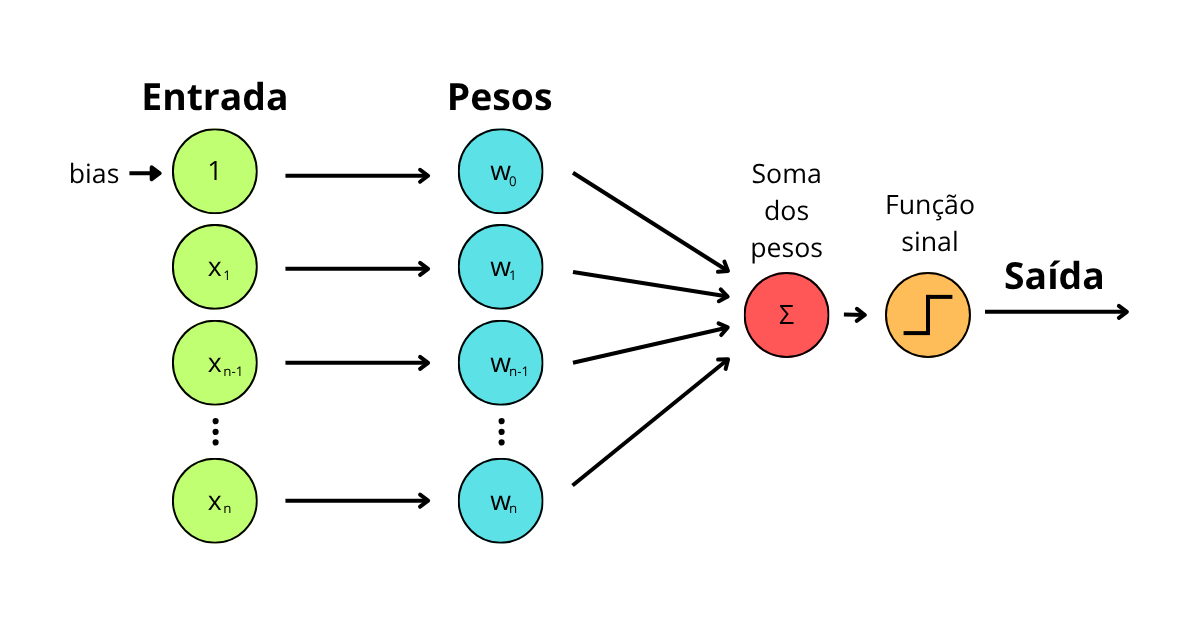
\includegraphics[width=1.0\textwidth]{images/perceptron.png}
	
	\vspace{5pt} % Espaçamento sutil entre a imagem e a fonte
	\centering
	\small Fonte: Elaborado pelo autor (2026).
\end{figure}

Contudo um perceptron por si só, não consegue resolver problemas não-lineares, afinal a combinação de entradas e saídas realizando uma operação linear não pode ter uma resposta para um problema não-linear. Mas a verdadeira solução para problemas não-lineares começa a partir da combinação de dois perceptrons. Intuitivamente, um perceptron é um classificador linear simples, mas combinando os resultados das respostas de dois perceptrons, que são lineares, com um terceiro neurônio combinando essas respostas, consegue resolver problemas não-lineares. Nesse contexto surge a ideia de redes.

Retomando o conceito de \citeonline{ghosh2023machine} entendemos o que são as redes, e o que são os nós, se tratam dos neurônios conectados e os pesos calculados de cada um. Contudo um conceito relevante que ainda não foi discutido, justamente esse conceito que permitiu a evolução do modelo de \citeonline{rosenblatt1958perceptron} para as redes multicamadas que existem hoje. O nome desse conceito é a retropropagação, conhecido também como \textit{backpropagation} que é justamente o que permite o aprendizado nessa arquitetura.

Após a invenção do perceptron havia ainda um espaço grande entre as redes neurais multicamadas e um único neurônio. O perceptron tem uma limitação relevante já citada, só consegue resolver problemas que são linearmente separáveis, isso acontece pela maneira como o aprendizado do modelo de \citeonline{rosenblatt1958perceptron} funciona. As entradas do perceptron eram multiplicadas com o peso e somadas com o viés, passada a uma função sinal ou degrau \footnote{A diferença dessas duas funções está na interpretação do 0, enquanto a função sinal tem a seguinte relação $sgn(x) \{-1\text{ se }x < 0; 0 \text{ se } x = 0; \text{ e } 1 \text{ se } x > 0$. Já a função degrau considera o 0 como um valor positivo $H(x) \{-1 \text{ se } x < 0; \text{ e } 1 se x >= 0$, ambas podem ser usadas no perceptron e ambas tem o mesmo problema que discutiremos no decorrer do texto} que resultava na saída. O aprendizado ocorria da seguinte forma: se a saída fosse igual a saída esperada, nenhum peso era alterado, se a saída fosse diferente da saída esperada os pesos eram modificados, até o modelo se ajustar a saída esperada.

Intuitivamente a limitação é explicita, mas para ficar mais evidente suponhamos o problema clássico das redes neurais, resolver o problema do ou-exclusivo, o XOR. A característica do XOR é que quando as entradas binárias são diferentes o resultado é 1, e quando as entradas são iguais o resultado é 0, conforme a tabela verdade: 

\begin{table}[htb]
	\centering
	\captionsetup{justification=centering}
	\caption{Tabela verdade da operação XOR}
	\label{tab:xor}
	\begin{tabular}{ccc}
		\hline
		A & B & $A \oplus B$ \\
		\hline
		0 & 0 & 0 \\
		0 & 1 & 1 \\
		1 & 0 & 1 \\
		1 & 1 & 0 \\
		\hline
	\end{tabular}
	\\[0.2cm]
	\footnotesize Fonte: Elaboração própria.
\end{table}

\citeonline{minsky1969introduction} provaram que o perceptron de \citeonline{rosenblatt1958perceptron} não conseguiria resolver um problema que não fosse linearmente separável, como o do XOR, imaginemos o XOR como um problema gráfico, enquanto um problema linear precisa de apenas uma reta para classificar corretamente os valores, para solucionar o XOR seriam necessários duas retas ou mais para classificar corretamente. E é exatamente nesse ponto em que o perceptron falha. A partir da constatação de \citeonline{minsky1969introduction} o mundo viveu uma era conhecida como o "inverno da IA", onde o modelo mais elegante criado até então ficaria estagnado.

Mas essa configuração mudou com a adoção de um método de aprendizado que mudou totalmente a forma como a \ac{ia} era construída, a retropropagação. A popularização do seu uso é atribuída a \citeonline{rumelhart1986learning} que aplicaram o conceito de retropropagação em redes neurais. "O procedimento ajusta repetidamente os pesos das conexões na rede para minimizar uma medida da diferença entre o vetor de saída real da rede e o vetor de saída desejado." \citem[p. 533, tradução nossa]{rumelhart1986learning}.

Esse marco inicia a construção dos modelos mais avançados de \ac{ia}, os modelos criados por  \citeonline{rumelhart1986learning} são redes neurais totalmente conectadas, significa que todos os neurônios de uma camada se conectam com os da camada seguinte. E baseada na  arquitetura do \textit{feedforward} em que os dados fluem em uma única direção da entrada para a saída, sem loops, ou recursão.

A elegância dessa solução é impressionante, porém aplicar ela a perceptrons combinados não é tão simples, existem algumas alterações do modelo de \citeonline{rosenblatt1958perceptron}. A primeira alteração é a noção de função de ativação, enquanto o perceptron utiliza a função sinal/degrau, a retropropagação não permite o uso desse tipo de função, essas funções não são deriváveis por serem descontinuas em x=0, e o conceito que permite a retropropagação é justamente o uso de derivadas, portanto a primeira alteração é a troca por uma função continua e derivável, como por exemplo a função sigmoide \footnote{Existem outras funções que podem ser usadas como ativação, como a ReLU (Unidade Linear Retificada), a TanH (Tangente Hiperbólica), a Softmax, a linear, etc. Não entraremos em detalhes sobre cada uma das funções de ativação, mas elas são uma das decisões que o pesquisador deve tomar ao usar redes neurais, o tipo de função de ativação, o número de camadas, a taxa de aprendizado são o que chamamos de hiperparametros do modelo, e o ajuste deles permite um desempenho melhor ou pior a depender dos dados e do problema.} representada na equação \ref{eq:sigmoide} e na figura \ref{fig:sigmoide}.


\begin{equation}
	\label{eq:sigmoide}
	f(x) = \dfrac{1}{1 + e^{-x}}
\end{equation}

\begin{figure}[h]
	\captionsetup{justification=centering}
	\caption{Função Sigmoide}
	\label{fig:sigmoide}
	\vspace{5pt}
	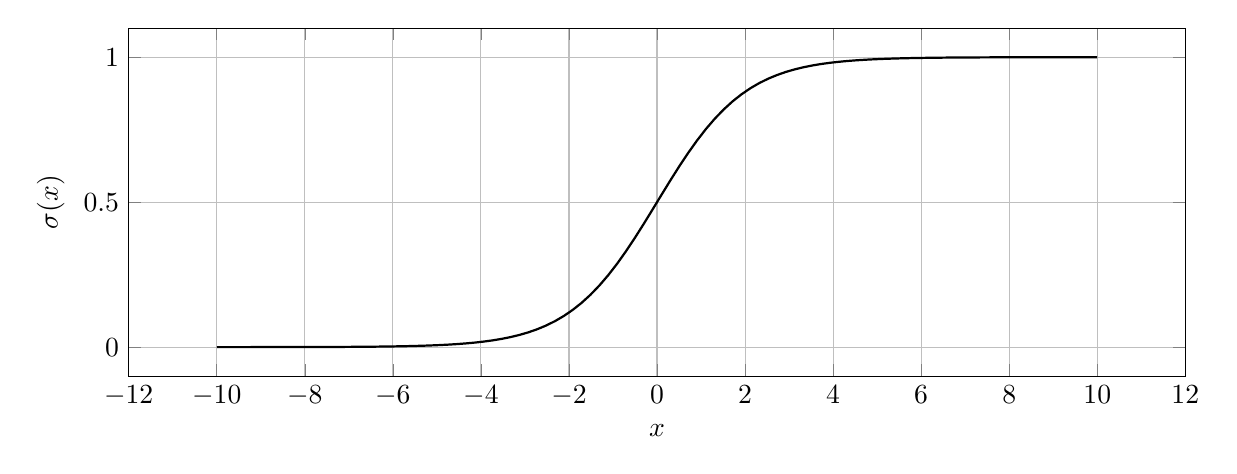
\begin{tikzpicture}
		\begin{axis}[
			xlabel={$x$},
			ylabel={$\sigma(x)$},
			domain=-10:10,
			samples=100,
			grid=major,
			width=15cm,
			height=6cm
			]
			\addplot[thick] {1/(1+exp(-x))};
		\end{axis}
	\end{tikzpicture}
	\vspace{5pt}
	\centering
	\small Fonte: Elaborado pelo autor (2026).
\end{figure}

A segunda alteração é a que permite a combinação dos neurônios, enquanto o perceptron usa o erro direto para recalcular os pesos, redes multicamadas essa noção não é direta. O erro da camada de saída deve ser utilizado para calcular os pesos da camada oculta anterior, com esses pesos calculados, calcular o erro da camada imediatamente precedente, e assim conseguinte até a primeira camada, esse processo é a retropropagação do erro, camada por camada. Esse processo é repetido inúmeras vezes até os pesos se ajustarem e o erro total for minimizado e é dessa maneira que a rede aprende.  

Mas como esse erro é minimizado? É com essa pergunta que conectamos com a necessidade da função de ativação ser derivável. Retomamos o conceito do calculo: A derivada mede a taxa de variação instantânea de uma grandeza em relação a outra, de uma forma geométrica a derivada representa a inclinação da reta tangente ao gráfico função em um ponto específico do plano. 

Nesse sentido o conceito de derivada para esse algoritmo funciona como uma bússola. Imaginemos que nossa função do erro é quadrática, como na equação \ref{eq:mse}, 


\begin{equation}
	E = \frac{1}{2}(y-\hat{y})^2
	\label{eq:mse}
\end{equation}

Onde:
\begin{itemize}
	\item $y$ representa o valor observado;
	\item $\hat{y}$ representa o valor predito;
	\item $E$ representa o erro quadrático.
\end{itemize}

A visualização dessa função pode ser verificado na figura \ref{fig:erroquadratico}.

\begin{figure}[htb]
	\centering
	\captionsetup{justification=centering}
	\caption{Função de erro quadrático.}
	\vspace{5pt}
	\label{fig:erroquadratico}
	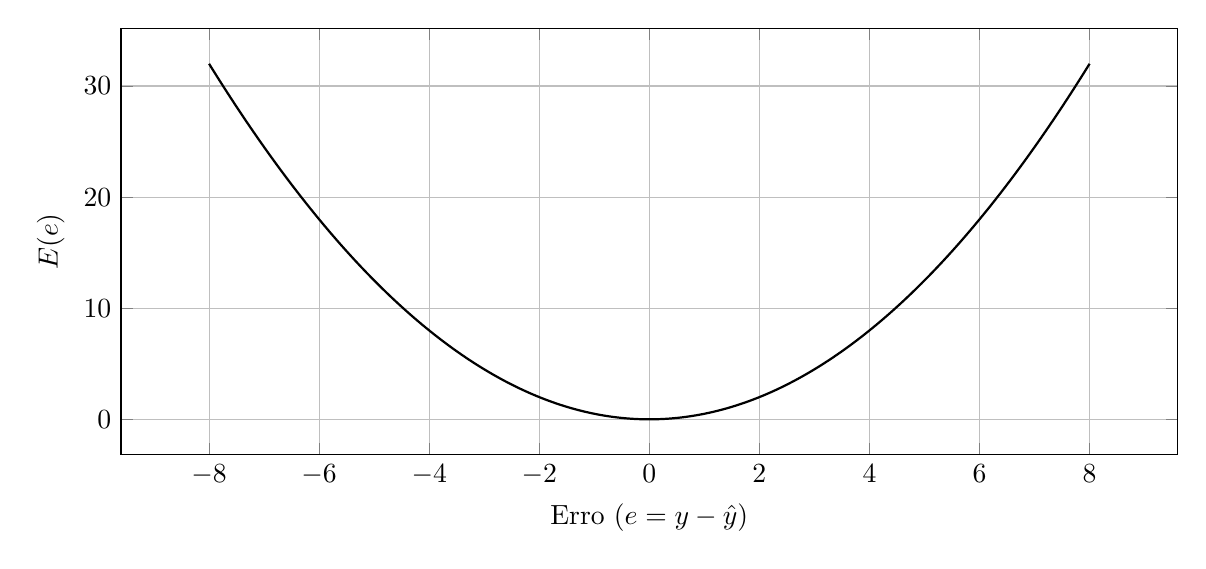
\begin{tikzpicture}
		\begin{axis}[
			xlabel={Erro ($e=y-\hat{y}$)},
			ylabel={$E(e)$},
			domain=-8:8,
			samples=200,
			grid=major,
			width=15cm,
			height=7cm
			]
			\addplot[thick] {0.5*x^2};
		\end{axis}
	\end{tikzpicture}

	\vspace{0.2cm}
	\footnotesize Fonte: Elaborado pelo autor (2026).
\end{figure}

Podemos usar o conceito da derivada para encontramos os valores de $\hat{y}$ que minimizam o erro $E$. Ajustando os coeficientes utilizando a derivada como ponteiro, procurando o melhor valor para que o erro seja minimizado, conforme a figura \ref{fig:gradiente_descendente_erro}.

\begin{figure}[htb]
	\centering
	\captionsetup{justification=centering}
	\caption{Função de erro quadrático e segmentos de retas tangentes representando o gradiente em diferentes pontos.}
	\vspace{5pt}
	\label{fig:gradiente_descendente_erro}
	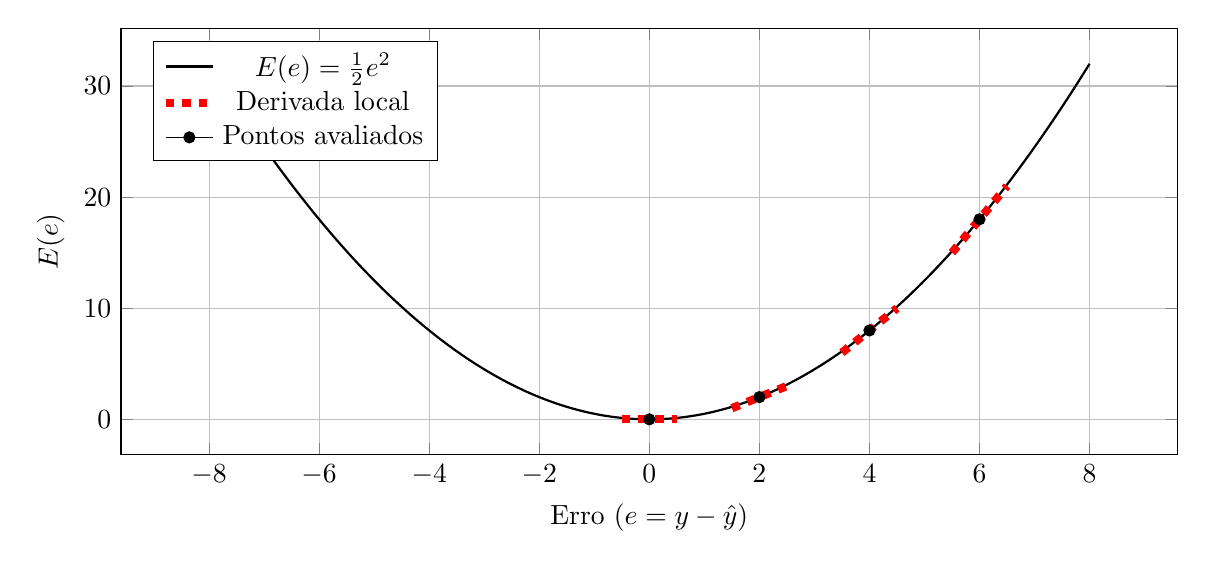
\begin{tikzpicture}
		\begin{axis}[
			xlabel={Erro ($e=y-\hat{y}$)},
			ylabel={$E(e)$},
			grid=major,
			width=15cm,
			height=7cm,
			legend pos=north west
			]
			
			% Função de erro
			\addplot[
			thick,
			domain=-8:8,
			samples=200
			] {0.5*x^2};
			\addlegendentry{$E(e)=\frac{1}{2}e^2$}
			
			% Ponto e=6
			\addplot[dashed, color=red, line width=3pt, domain=5.5:6.5] {6*(x-6)+18};
			\addlegendentry{Derivada local}
			\addplot[mark=*] coordinates {(6,18)};
			\addlegendentry{Pontos avaliados}
			
			% Ponto e=4
			\addplot[dashed, color=red, line width=3pt, domain=3.5:4.5] {4*(x-4)+8};
			\addplot[mark=*] coordinates {(4,8)};
			
			% Ponto e=2
			\addplot[dashed, color=red, line width=3pt, domain=1.5:2.5] {2*(x-2)+2};
			\addplot[mark=*] coordinates {(2,2)};
			
			% Ponto e=0
			\addplot[dashed, color=red, line width=3pt, domain=-0.5:0.5] {0};
			\addplot[mark=*] coordinates {(0,0)};
			
		\end{axis}
	\end{tikzpicture}

	
	\vspace{0.2cm}
	\footnotesize Fonte: Elaborado pelo autor (2026).
\end{figure}

Porém a função de erro de uma rede neural não é uma simples função quadrática, afinal se fosse a solução seria trivial, o gráfico seria algo mais parecido com o representado na figura \ref{fig:superficie_erro}, mas mesmo assim a representação é imprecisa, pois redes neurais profundas contam com muitas entradas e camadas, possuem n-dimensões e é praticamente impossível conceber uma representação visual do erro dessas redes. Porém, mesmo que imprecisas, essas representações nos permitem entender a ideia por trás da retropropagração, o chamado gradiente descendente.

\begin{figure}[htb]
	\centering
	\captionsetup{justification=centering}
	\caption{Superfície de erro}
	\label{fig:superficie_erro}
	\vspace{5pt}
	
	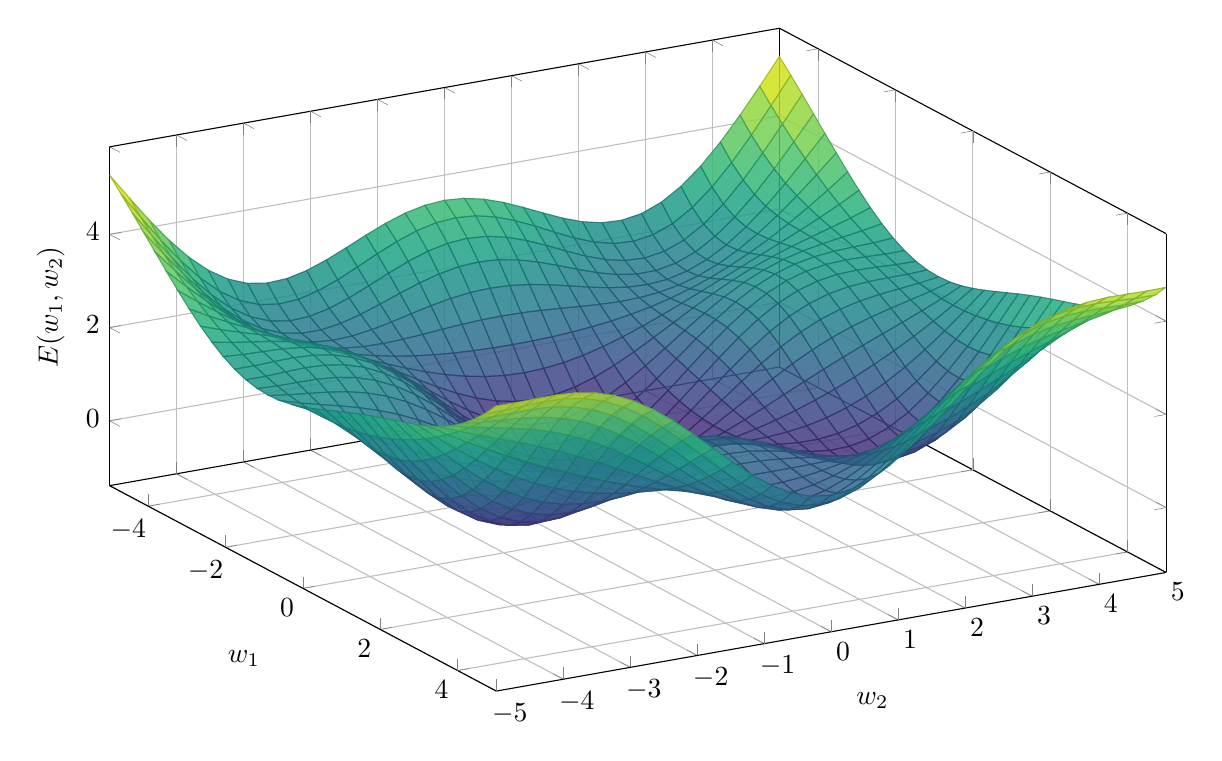
\begin{tikzpicture}
		\begin{axis}[
			view={60}{35},
			width=15cm,
			height=10cm,
			xlabel={$w_1$},
			ylabel={$w_2$},
			zlabel={$E(w_1,w_2)$},
			colormap/viridis,
			grid=major
			]
			
			% Superfície de erro
			\addplot3[
			surf,
			opacity=0.85,
			samples=35,
			domain=-5:5,
			y domain=-5:5
			]
			{0.1*(x^2+y^2)+sin(deg(x))*cos(deg(y))};
			
		\end{axis}
	\end{tikzpicture}
	

	\vspace{0.2cm}
	\footnotesize Fonte: Elaborado pelo autor (2026).
	
\end{figure}

O gradiente descendente "É um método iterativo no qual começamos com um palpite inicial da solução e depois refinamos gradualmente." \citem[p. 45, tradução nossa]{ekman2021learning}. Para funções simples de uma variável o gradiente descendente é o algoritmo que usa as derivadas das funções para minimizar o erro, por outro lado

\begin{citacao}
	Se tivermos uma função de n variáveis, então nosso gradiente consistirá em n derivadas parciais, e podemos calcular o próximo passo como $x-\eta \nabla y$, onde tanto $x$ quanto $\nabla y$ são vetores com $n$ elementos.  \citem[p. 47, tradução nossa]{ekman2021learning}
\end{citacao}

Uma maneira mais intuitiva de se entender o gradiente descendente seria com uma analogia: O gradiente descendente é como um animal cego e com sede encima de um terreno acidentado, ele não sabe onde tem água, e não sabe onde está, porém ele sabe que a água fica nos vales, e pode usar suas patas para identificar a inclinação do terreno, ele procurará maneiras de sempre ir descendo, e quando chegar no vale encontrará água.

E com essa analogia já entendemos também um dos problemas dessa arquitetura, os mínimos locais. Se o animal encontra uma depressão na montanha, que não tem água, mas que para todos os lados é necessário subir primeiro para posteriormente descer o animal cego acaba morrendo de sede. De certa forma é assim que funciona o gradiente descendente, quando encontra mínimos locais, o algoritmo "pensa"\, estar na solução ótima, mas é apenas um mínimo local\footnote{Existem estudos dedicados a minimizar esses problemas, como encontrar uma taxa de aprendizado ótimo, para evitar mínimos locais e mesmo assim encontrar soluções adequadas, mas essas análises fogem do escopo de nosso trabalho, mas vale a leitura do livro de  \citeonline{ekman2021learning} para entender mais sobre redes neurais, funções de ativação, gradiente descendente e outros conteúdos sobre redes neurais na teoria e na prática}.

% Ainda estou pensando se coloco a parte de algebra linear no texto para falar sobre a formulação matemática, vou perguntar para o professor

Com essa noção de como surgiram os modelos baseados em redes neurais, posteriormente com a evolução das técnicas de \ac{ia} surgem os algoritmos de \textit{deep learning} (aprendizado profundo), esses modelos não são ão diferentes das redes neurais estudadas no presente trabalho, a principal diferença é a escala. No \textit{deep learning} são muitas camadas, imagine da seguinte forma com zero camadas ocultas temos uma regressão logística ou um perceptron, com uma camada oculta temos as redes neurais, com duas ou mais temos o que chamamos de \textit{deep neural networks} que são redes neurais com muitas camadas ocultas. Esses algoritmos que rodam as grandes tecnologias de \ac{ia} hoje, como visão computacional e chatbots, contudo também apresentam um dos problemas desse tipo de técnica e do aprendizado de máquina de uma forma geral, a interpretabilidade.

Redes com arquiteturas gigantescas podem resolver problemas complexos, porém não tem a interpretabilidade que modelos simples possuem. 

A partir desse exposto vimos de uma forma simplificada como redes neurais surgiram e como elas funcionam por baixo dos panos, agora podemos ver as aplicações desses modelos para predição econômica.

Começaremos por \citeonline{vasconcelos2017poder} que utilizou modelos de redes neurais em sua tese, diferente de nosso trabalho o autor realizou sua pesquisa em dados de 41 países de 2001 à 2015 (Segundo o autor em alguns casos a séria pode até ser mais extensa devido a disponibilidade), essa escolha se deu principalmente por serem membros da \ac{ocde}, mais alguns países que apesar de não serem membros possuem relevância econômica e/ou tinham a disponibilidade de dados.

As variáveis selecionadas pelo autor são: pib, seus componentes, comércio internacional, preços, câmbio, juros, títulos públicos, câmbio, mercado futuro, índices de bolsa, demais indicadores de negócios público e privado, qualidade do crédito, operações de crédito do governo em detalhes, operações financeiras como BIS, reservas, balança comercial, fluxo de capitais, CDS\footnote{\textit{Credit Default Swap} que é um indicador de risco de crédito.}, VIX\footnote{Índice de volatilidade.}, preços de commodities. Essas variáveis\footnote{Para mais detalhes sobre as variáveis recomendamos a consulta do material original de \citeonline{vasconcelos2017poder}} são de frequência trimestral. Os dados foram coletados a partir de conjunto de bases (Banco Mundial, \ac{ocde}, BIS, Bloomberg)

O autor comparou diversos modelos nesse teste, modelos de equações individuais, Fatores comuns, modelos mistos de quadrados mínimos ordinários, Lasso e regressão em árvore e métodos de \textit{machine learning} como \textit{Suport Vector Machine}, \textit{Random Forest}  e \textit{deep learning}.

O objetivo do autor era verificar as relações entre Política fiscal, mercado internacional e as flutuações do produto dos países, no sentido de desempenho o autor constatou que os modelos baseados em \textit{deep learning} conseguiram superar os modelos tradicionais de equações individuais e de fatores comuns, porém se saíram piores que os modelos mistos construídos, assim como teria se saído pior que os outros modelos de \textit{machine learning} analisados na tese.

No sentido todos os modelos apontaram a interpretação de que o mercado internacional foi mais determinante do que a política fiscal. O autor aponta que redes neurais são sim métodos robustos para predição de modelos macroeconômicos. Porém conforme os resultados apontados fica evidente que redes neurais tem falhas estruturais como a interpretabilidade e não são necessariamente a melhor solução para todos os problemas.

\citeonline{carmo2023modelagem} também comparou modelos, eles os classificaram entre clássicos e contemporâneos. O trabalho examinou dois modelos: regressão linear simples; e redes neurais multicamadas. Assim aplicaram ambos modelos à predição da remuneração média mensal paga 
aos empregados nas 27 unidades da federação brasileira. Para isso os dados foram extraídos do \ac{ibge} através do \ac{sidra}. O estudo aponta um desempenho superior das redes neurais em comparação a regressão linear no critério da precisão. Contudo, os autores levantaram o mesmo ponto de \citeonline{vasconcelos2017poder} que a interpretabilidade das redes neurais é limitada. 

\begin{citacao}
	Do ponto de vista analítico, a análise de regressão linear é mais dinâmica e informativa que a RNA MLP\footnote{Redes Neurais Artificiais \textit{Multilayer Perceptron}}. Pois, ao identificar os coeficientes do modelo de regressão e seus sinais, é possível compreender o impacto de cada variável independente significativa na explicação do comportamento da variável de estudo. Ao passo que, a RNA MLP somente permite avaliar qual o grau de importância das variáveis  explicativas do modelo. \citem[p. 17]{carmo2023modelagem}
\end{citacao}

\citeonline{carmo2023modelagem} demonstraram que as redes neurais possuem uma capacidade modelar todas as variáveis, enquanto outros métodos como a regressão linear só consideram as variáveis significantes para o modelo. Outro ponto elencado pelos autores é a capacidade de modelar problemas não lineares, sendo uma vantagem em relação so modelo tradicional da regressão linear.

Os autores pontuam que ambos métodos tem vantagens e desvantagens, enquanto modelos tradicionais possuem rigor metodológico e capacidade interpretativa, modelos contemporâneos, como redes neurais podem ser considerada mais flexíveis, adaptando-se a tendências não-lineares, e até a dados incompletos, porém devido a sua complexidade arquitetural possuem baixa interpretabilidade.

\citeonline{amaral2023previsao} também realizaram testes de modelos baseados em redes neurais, porém ao invés de comparar a outras técnicas tradicionais, os autores testaram diferentes configurações de redes neurais. A principal diferença dos modelos até então apresentados é o métodos de treinamento, enquanto as redes neurais estudadas são do tipo totalmente conectada baseadas no \textit{feedfoward} as três redes testadas por \citeonline{amaral2023previsao} são do tipo \ac{rnn}\footnote{Redes Neurais Recorrentes}.

\begin{citacao}
	As \ac{rnn} são um tipo de rede neural que foi 
	desenvolvida para identificar padrões em um banco de dados. Através dos algoritmos da rede neural, ele é capaz de identificar, dentro de uma sequência de informações, similaridades de palavras, de texto, imagens e números, utilizando esses padrões para aprender e futuramente entender o que o está sendo “apresentado”. \citem[p. 11]{amaral2023previsao}
\end{citacao}

Para além disso os autores utilizaram um tipo de \ac{rnn} mais sofisticada, a chamada \ac{rnn} de Memória \ac{lts}, segundo os autores na arquitetura desse tipo de \ac{rnn} é possível armazenar memórias de longo e curto prazo. Sendo uma arquitetura adequada para séries temporais econômicas que sofrem influências de curto e longo prazo.

No trabalho os autores testaram três modelos de redes neurais: univariado \textit{stacked}\footnote{Esse tipo de modelo "possui uma arquitetura de mais de uma camada de neurônio escondida, no qual cada camada contém múltiplas células de memória." \citem[p. 13]{amaral2023previsao}.}; multivariado; e univariado bidirecional\footnote{Em modelos Univariados bidirecionais, ao invés de um único modelo, existem dois. O primeiro aprende a sequência da entrada e o segundo o inverso, proporcionando um maior quantitativo de informações para o treinamento. \citem{amaral2023previsao}}. Os dados foram extraídos do banco central do Brasil e do \ac{ibge} no período de janeiro de 2002 até março de 2023. O conjunto de dados compreende: taxa SELIC\footnote{\ac{selic}}; IPCA\footnote{\ac{ipca}}; PIM\footnote{\ac{pim}}; e taxa de câmbio.

Os resultados apontados pelos autores indicaram um desempenho relevante das \ac{rnn} \ac{lts}. O melhor dos três modelos foi o multivariado, que apresentou os menores indicadores de erros, possuindo um maior grau de explicabilidade. O segundo com melhor desempenho foi o modelo univariado \textit{stacked}, em que os modelos que usaram a taxa \ac{selic} como entrada, obtiveram os melhores resultados. E o pior dos modelos foi o univariado bidirecional, que não obteve resultados satisfatórios, não superando em nenhuma variável o modelo univariado \textit{stacked}.

A reflexão proposta pelo autor é que mesmo com uma quantidade limitada de dados o modelo baseado em \ac{rnn} \ac{lts} multivariado teve desempenho satisfatório para predição de variáveis econômicas. Mas que mesmo o modelo obtendo um resultado aceitável, ainda assim é necessário uma análise de indicadores históricos e fáticos por um profissional técnico da área.

A partir do exposto de \citeonline{amaral2023previsao} foi possível notar outro tipo de arquitetura para redes neurais, essa com uma adequação relevante para séries históricas, porém ainda assim com as limitações inerentes a esse tipo de modelo, que apesar de terem uma explicabilidade alta dos fatores envolvidos no modelo e uma capacidade de captar relações quase que imperceptíveis nas variáveis econômicas, ainda se faz necessário o aval do técnico economista, implicando que a interpretabilidade de um modelo é algo imprescindível.

Como nos outros modelos, é importante olhar como a literatura internacional utiliza os modelos. Entretanto, dessa vez, vamos utilizar o material de \citeonline{ghosh2023machine}, que realizaram um trabalho com redes neurais para predição do \ac{gdp} da Índia de janeiro de 2003 a dezembro de 2019. Esse material se assemelha com o que desejamos produzir com o presente trabalho, claro por tratarem de uma série histórica semelhante, mas especialmente pois tanto o Brasil como a Índia são membros da lista de países emergentes, o que implica em economias complexas com características parecidas.

Os dados do trabalho foram extraídos do Banco da Reserva da Índia ou da CEIC\footnote{Trata-se de uma base de dados de indicadores macroeconômicos globais}, foram analisadas 13 variáveis mais o \ac{gdp} como variável a ser predita. O modelo proposto pelos pesquisadores da Índia tratava-se de uma combinação de modelos para o \textit{nowcasting}\footnote{\textit{nowcasting} é uma técnica de predição de variáveis de alta frequência, no contexto do estudo predizer o \ac{gdp} usando variáveis diárias/semanais}, o modelo principal é um \ac{dfm}, como visto anteriormente, para estimar valores para cada indicador econômico com base nos valores históricos desses indicadores foram utilizados três varições de modelo: \textit{Random Forest}, ARIMA, Prophet\footnote{O modelo Random Forest ainda veremos mais sobre o mesmo no presente trabalho. O modelo Prophet não será contemplado profundamente, mas afim de curiosidade esse é um procedimento baseado em modelos aditivos com ampla capacidade para aplicação em \textit{nowcasting} por conseguir ajustar tendências não-lineares usando a sazonalidade \citem{ghosh2023machine}.}. E como modelo ponte, que conecta os fatores dinâmicos estimados com o \ac{gdp}, temos o AR(1) e as redes neurais.

Os resultados obtidos pelos pesquisadores apontam que o modelo Prophet se saiu melhor no \textit{nowcasting} do \ac{gdp}, e que para previsões a partir de um mês as redes neurais apresentaram uma melhoria significativa em relação ao modelo AR(1), mas que para longos períodos, mais de um ano, o erro só aumentou, indicando que esse tipo de modelo de \textit{nowcasting} não é o mais indicado para predição em longos períodos.

Apesar da semelhança dos dados e do contexto de aplicação, o trabalho de \citeonline{ghosh2023machine} busca um outra técnica de predição, buscando a alta frequência das variáveis e informações rápidas para tomadas de decisões fundamentadas. A partir do exposto dos autores é possível notar como diferentes modelos podem ser combinados para encontrar a melhor solução, nesse contexto as redes neurais foram usadas como modelo ponte, não como modelo principal, mas mesmo assim obtiveram resultados melhores que um modelo consolidado como o AR(1) para o \textit{nowcasting}.

A partir dessa exposição de autores fica claro como métodos atuais como as redes neurais tem ganhado espaço dentro da predição econômica, não se tratam de modelos milagrosos que conseguem resolver todos os problemas do mundo. Esses modelos tem sim uma liberdade maior, não se restringindo a metodologias rígidas conforme \citeonline{carmo2023modelagem}, mas ainda assim dependem de um pesquisador o conduzindo e interpretando seus resultados \citem{amaral2023previsao}.

Vimos também que talvez sua maior potencialidade não seja como o perceptron de \citeonline{rosenblatt1958perceptron}, mas sim a combinação com outras técnicas e variações, criando modelos com alta capacidade preditiva e robustez conforme \citeonline{amaral2023previsao} e \citeonline{ghosh2023machine} demonstraram.


















 






\subsubsection{Florestas Aleatórias}

%\citeonline{kava2022alem} e de \citeonline{rebelo2022interpretabilidade} que

%Diante desse contexto optamos por apresentar os modelos de uma maneira didática, do mais "fácil" ao mais "difícil", isso é um juízo de valor bem subjetivo, contudo para construção de uma sequência lógica possível de acompanhar, descrever os modelos em grau de complexidade, parece ser uma boa alternativa para um texto compreensível.
%
%Certamente o grau de complexidade de um modelo está relacionado a quantidade de variáveis usadas, assim como o quão trabalhoso é para se aplicar esse modelo, nesse sentido o ARIMA, talvez seja um dos modelos preditivos mais simples.

%O ARIMA, ou em português, modelo auto-regressivo de médias móveis, é um modelo que utiliza da pr



% EU QUERO COLOCAR OS TESTES, MAS SE NÃO DER TEMPO NÃO COLOCAREI NA QUALIFICAÇÃO

%\section{Testes: Comprovar e comparar modelos}
%\label{sec:testes}


%	\citem{laudon2022sistemas} sistemas de informação são essenciais para alcançar objetivos estratégicos dos negócios. Na era digital, o grande volume de dados gerados pelos sistemas de informação pode ser usada como uma fonte, praticamente inesgotável de informações para tomadas de decisões. 
%
%	Rever trabalhos sobre uso dessas técnicas para predição


% NÃO SEI SE IREI COLOCAR ESSA SESSÃO, MAS PENSO QUE SIM
%\section{IA vs Tradicional: Uma perspectiva Acadêmica}
    \chapter{Metodologia}
\label{chap:metodologia}

\section{Delineamento de pesquisa}
Com base nos objetivos da presente pesquisa, a mesma se classifica como explicativa. Esse tipo de pesquisa "têm como preocupação central identificar os fatores que determinam ou que contribuem para a ocorrência dos fenômenos." \citem[p. 87]{Gil}. Ao analisarmos o desempenho dos diferentes modelos econométricos voltados para a predição do PIB brasileiro, estamos buscando identificar e compreender os diferentes fatores que explicam esse desempenho, enquadrando-a como explicativa.

Sobre os procedimentos de coleta de dados, a presente pesquisa se enquadra como documental, por utilizar-se de dados que não receberam um tratamento e estão dispostos em repositórios digitais de dados. Segundo \citeonline{Gil} a pesquisa documental apropria-se de diversas fontes, não somente material impresso em bibliotecas, onde os documentos utilizados podem ter um tratamento analítico ou não.

Por fim, ao se tratar de uma pesquisa que compara diferentes modelos econométricos, assim como avalia o desempenho dos mesmos, seguindo o rigor matemático e estatístico, ela se enquadra como uma pesquisa predominantemente quantitativa onde apropria-se do método comparativo e estatístico. Para \citeonline{LAKATOSMARCONI} o método estatístico trata-se da redução dos fenômenos a termos quantitativos e a manipulação estatística, onde possibilita a generalizações sobre sua natureza, ocorrência ou significado. Já "o método comparativo é usado tanto para comparações de grupos." \citem[p. 107, 108]{LAKATOSMARCONI}.


%	Aqui eu tenho que falar sobre os objetivos
%	O procedimento de coleta
%	Quanto a abordagem as questões de Pesquisa
\section{Procedimento de coleta de dados}

As variáveis foram escolhidas baseadas na dissertação de \citeonline{rebelo2022interpretabilidade}, descritas mais evidentemente na sessão \ref{cap:revisao-literatura}. As variáveis escolhidas podem ser verificadas na tabela \ref{tab:fontes_dados}. Os dados utilizados na pesquisa foram extraídos de duas APIs (\textit{Application Programming Interface}, no português, Interface de programação de aplicações). A relação variável - Fonte - URL da API pode ser vericada na mesma tabela.

A primeira fonte foi a API de dados agregados do IBGE, onde nela existem informações econômicas, sociais e demográficas do Brasil. 


\begin{citacao}
	O IBGE possui uma Application Program Interface (API) de serviços de dados abertos que disponibiliza dados processáveis por máquina para qualquer cidadão ou sistema, permitindo a interoperabilidade e o enriquecimento a partir dos dados abertos disponibilizados. \citem[p. 2]{silva2024dados}.
\end{citacao}

A segunda API utilizada foi a API do BACEN (Banco Central do Brasil), onde foram extraídos dados financeiros. Segundo o próprio \citeonline{bcb_dados_abertos} o "catálogo de dados, permite que os usuários encontrem os conjuntos de informações de seu interesse, entendam sua estrutura e suas limitações, e tenham acesso ao caminho para os dados."

O período analisado foi de 2007 à 2022, devido a disponibilidade de datas nas bases de dados. 

\begin{table}
	\centering
	\caption{Fontes de dados utilizadas nas APIs do IBGE e BACEN}
	\label{tab:fontes_dados}
	\resizebox{\textwidth}{!}{
		\begin{tabular}{p{4cm} p{2cm} p{9cm}}
			\hline
			\textbf{Indicador} & \textbf{Fonte} & \textbf{URL / Endpoint da API} \\
			\hline
			PIB & IBGE & \small \url{https://servicodados.ibge.gov.br/api/v3/agregados/6784/periodos/-20/variaveis/9808?localidades=N1[all]} \\
			Deflator do PIB & IBGE & \small \url{https://servicodados.ibge.gov.br/api/v3/agregados/6784/periodos/-20/variaveis/9811?localidades=N1[all]} \\
			população (milhões) & IBGE & \small \url{Ainda nao coletado} \\
			índice de direitos de propriedade & IBGE & \small \url{Ainda nao coletado} \\
			índice de eficiência jurídica & IBGE & \small \url{Ainda nao coletado} \\
			índice de integridade governamental & IBGE & \small \url{Ainda nao coletado} \\
			índice de despesa governamental  & IBGE & \small \url{Ainda nao coletado} \\
			despesa pública em educação (\% PIB) & IBGE & \small \url{Ainda nao coletado} \\
			despesa pública em saúde (\% PIB) & IBGE & \small \url{Ainda nao coletado} \\
			despesa pública em proteção ambiental (\% PIB) & IBGE & \small \url{Ainda nao coletado} \\
			índice de carga fiscal & IBGE & \small \url{Ainda nao coletado} \\
			índice de saúde fiscal  & IBGE & \small \url{Ainda nao coletado} \\
			dívida publica (\% PIB) & IBGE & \small \url{Ainda nao coletado} \\
			índice de liberdade empresarial & IBGE & \small \url{Ainda nao coletado} \\
			índice de liberdade laboral & IBGE & \small \url{Ainda nao coletado} \\
			taxa de desemprego & IBGE & \small \url{Ainda nao coletado} \\
			índice de liberdade monetária  & IBGE & \small \url{Ainda nao coletado} \\
			taxa de inflação  & IBGE & \small \url{Ainda nao coletado} \\
			índice de liberdade comercial & IBGE & \small \url{Ainda nao coletado} \\
			balança corrente  & IBGE & \small \url{Ainda nao coletado} \\
			Taxa aduaneira & IBGE & \small \url{Ainda nao coletado} \\
			índice de liberdade investimento  & IBGE & \small \url{Ainda nao coletado} \\
			investimento direto estrangeiro (\% PIB) & IBGE & \small \url{Ainda nao coletado} \\
			índice de liberdade financeira & IBGE & \small \url{Ainda nao coletado} \\
			\hline
		\end{tabular}
	}
\end{table}




\section{Procedimento de análise de dados}

A análise dos dados é um processo muito importante ao usar modelos matemáticos, conforme \citeonline{MoniqueGIGO} a qualidade das respostas depende diretamente dos dados usados 
\footnote{O termo coloquial em inglês para essa situação se chama GIGO ou \textit{Garbage In Garbage Out}, que em tradução livre - lixo entra lixo sai.}.
Ou seja, não basta ter fontes confiáveis como o \citem{bcb_dados_abertos} e o \citem{ibge_api}, é necessário um procedimento confiável de ponta a ponta.
Para esse processamento dos dados, foi utilizado a linguagem de programação \textit{Python}
\footnote{Python é amplamente utilizado em computação científica e numérica \citem{python}}
e suas bibliotecas.


O primeiro processo de tratamento foi a conversão dos tipos nativos das APIs para um formato adequado para análise com Python, isso foi feito através da biblioteca Pandas. "Pandas é uma biblioteca de Python de estruturas de dados e ferramentas estatísticas, inicialmente desenvolvida para aplicações de finanças quantitativas." \citem[p. 1, \textit{tradução nossa}]{mckinney2010pandas}.

O segundo passo de tratamento foi a inflação dos dados para 2022, último ano da série, isso foi feito através de um índice de preços, que pode verificado na equação \ref{eq:inflacao}. O \citeonline{ibge_pib_series} traz a definição de deflator do PIB, porém que se aplica as demais variáveis, em que um deflator é a variação do valor corrente da variável no tempo $(t)$ em relação ao valor da varável do ano $(t)$ a preços do ano anterior, ou seja a variação percentual em relação ao mesmo período do ano anterior.
\begin{equation}
	\label{eq:inflacao}
	\text{Valor real} = \frac{\text{Valor Nominal}}{\text{índice de Preços}} \times 100
\end{equation}

O terceiro passo de tratamento foi o treinamento dos modelos. Nesse passo foram utilizados as bibliotecas Scikit-learn e Tensorflow, os modelos foram treinados com dados de 2007 à 2017, totalizando 10 anos na série histórica (dados de treinamento), e deixando os últimos 5 anos (2017 à 2022) para a testagem dos resultados do modelo. Para \citeonline{santos2022previsao} as eficácias dos modelos nos dados de treinamento não são importantes, o que é relevante é como o modelo se sai com os dados de teste, ou seja, se o modelo consegue ser extensivo no período fora da amostra.

O último passo foi o cálculo das métricas de avaliação dos modelos, para esse passo foram avaliadas três dimensões: acurácia, interpretabilidade e custo computacional.

Para a acurácia foram escolhidas as métricas que foram utilizadas por \citeonline{rebelo2022interpretabilidade}: o  Erro Quadrático Médio (EQM) descrito na equação \ref{eq:EQM}; Erro Absoluto Médio (EAM) descrito na equação \ref{eq:EAM}; a Raiz do Erro Quadrático Médio (REQM) descrito na equação \ref{eq:REQM}; e por fim, o erro percentual absoluto médio (EPAM) descrito na equação \ref{eq:EPAM}.

\begin{equation}
	\label{eq:EQM}
	\text{EQM} = \frac{1}{n}\sum_{i=1}^{n}(y_i \hat{y_i})^2
\end{equation}

\begin{equation}
	\label{eq:EAM}
	\text{EQM} = \frac{1}{n}\sum_{i=1}^{n}|y_i \hat{y_i}|
\end{equation}

\begin{equation}
	\label{eq:REQM}
	\text{REQM} = \sqrt{\text{EQM}}
\end{equation}

\begin{equation}
	\label{eq:EPAM}
	\text{EPAM} = \frac{1}{n}\sum_{i=1}^{n}|\frac{y_i \hat{y_i}}{y_i}| \times 100
\end{equation}

Para \citeonline{kava2022alem} a interpretabilidade está diretamente relacionada a facilidade que um ser humano tem de entender os resultados de um modelo. Para essa dimensão foram usadas as métricas: Efeitos Locais Acumulados (ELA) descrito na equação \ref{eq:ELA}; e a interação ente preditores através da estatística-H, descrita na equação \ref{eq:H}, ambas descritas por \citeonline{kava2022alem}.

\begin{equation}
	\label{eq:ELA}
	\tilde{f}_j,\text{ELA}(x) = \sum_{k=1}^{k_j(x)}\frac{1}{n_k(k)} \sum_{i:X_j \in N_j(k)}[\hat{f}(z_{k,j},x_j^{(i)})-\hat{f}(z_{k-1,j},x_j^{(i)})]
\end{equation}



\begin{equation}
	\label{eq:H}
	H_j^2 = \frac{ \sum_{i=1}^{n}[\hat{f}(x^{(i)})-PD_J(X_J^{(I)})-PD_{-J}(X_{-J}^{(I)})]^2}{\sum_{i=1}^{n}\hat{f^2}(x^{(i)})}
\end{equation}

A última dimensão é o custo computacional, essa se baseará principalmente no tempo de execução dos modelos, e na contagem de operações com ponto flutuantes - FLOPs (do inglês, FLOating Point Operations) em ambas as métricas, quanto mais alto o valor, maior é o custo computacional.


\section{Constructo da pesquisa}
A estrutura do constructo pode ser verificado na tabela \ref{tab:Constructo}
%	\begin{table}
	%		\centering
	%		\caption{Constructo da pesquisa}
	%		\label{tab:Constructo}
	%		\begin{tabular}{p{2cm} p{4cm} p{9cm}}
		%			\hline
		%			\textbf{Objetivo} & \textbf{Onde analisar} & \textbf{Como analisar}\\
		%			a & Revisão de literatura & Levantar na literatura os principais modelos econométricos tradicionais (VAR, ARIMA, DFM e MIDAS) e de IA aplicados à predição do PIB \\ 
		%			a & Revisão de literatura & Descrever cada modelo identificado, apresentando suas formulações algébricas e funcionais \\ 
		%			b & Revisão de literatura & Identificar na literatura as variáveis determinantes na estimativa do PIB \\ 
		%			b & Metodologia & Selecionar e justificar as variáveis que serão utilizadas, bem como suas respectivas fontes de dados \\ 
		%			c & Análise e Discussão dos resultados & Aplicar os modelos econométricos e de IA utilizando as variáveis selecionadas para estimar o PIB \\ 
		%			c & Análise e Discussão dos resultados & Calcular as métricas de desempenho (acurácia, interpretabilidade e custo computacional) de cada modelo \\ 
		%			d & Análise e Discussão dos resultados & Comparar os resultados obtidos entre os modelos de IA e os modelos econométricos tradicionais \\ 
		%			d & Conclusão & Discutir criticamente o desempenho dos modelos e destacar suas vantagens e limitações em cada dimensão de avaliação \\ 
		%			\hline
		%		\end{tabular}
	%	\end{table}
\begin{table}[H]
	\centering
	\caption{Constructo da pesquisa}
	\label{tab:Constructo}
	\begin{tabular}{p{14.5cm}}
		\hline
		\textbf{Pergunta de Pesquisa} \\
		\hline
		Em que medida modelos preditivos baseados em \ac{ia}, comparados aos modelos tradicionais VAR, ARIMA, DFM e MIDAS, conseguem estimar o PIB brasileiro? \\
		\hline
		\textbf{Objetivo Geral} \\
		\hline
		Analisar em que medida modelos preditivos baseados em \ac{ia}, comparados aos modelos tradicionais VAR, ARIMA, DFM e MIDAS, conseguem estimar o PIB brasileiro.
	\end{tabular}
	\resizebox{\textwidth}{!}{
		\begin{tabular}{p{4cm} p{5.0cm} p{3.5cm} p{4.6cm}}
			\hline
			\textbf{Objetivos específicos} & \textbf{variáveis/dados à coletar} & \textbf{Como analisar} & \textbf{Fonte}. \\
			\hline
			Caracterizar os modelos econométricos tradicionais (VAR, ARIMA, DFM e MIDAS) e de IA para a predição do PIB. & Modelos econométrico com capacidade de predizer séries temporais. & Buscar através da literatura modelos já utilizados com esses fins. & \citeonline{castelli2022modelo}, \citeonline{azevedo2020modelagem}, \citeonline{azevedo2020modelagem}, \citeonline{ciquini2023modelo}, \citeonline{silva2024dados}, \citeonline{alves2009nucleo}, \citeonline{moura2020fragilidade} e \citeonline{micheletti2024avaliaccao}. \\
			\hline
			Identificar as diferentes variáveis determinantes na estimativa do PIB. & Variáveis com possível influência no PIB com facilidade de coleta e atualização recorrente. & Procurar na literatura quais variáveis são utilizadas para a predição do PIB. & \citeonline{rebelo2022interpretabilidade}, \citeonline{ibge_api} e \citeonline{bcb_dados_abertos}. \\
			\hline
			Aplicar diferentes modelos econométricos tradicionais e de IA para a predição do PIB. & Modelos econométricos e variáveis encontradas nos primeiros dois objetivos. & treinar os diferentes modelos usando os dados coletados através da linguagem de programação Python e suas bibliotecas de estatística.  & \citeonline{castelli2022modelo}, \citeonline{azevedo2020modelagem}, \citeonline{azevedo2020modelagem}, \citeonline{ciquini2023modelo}, \citeonline{silva2024dados}, \citeonline{alves2009nucleo}, \citeonline{moura2020fragilidade} e \citeonline{micheletti2024avaliaccao}.\\
			\hline
			Comparar o desempenho dos modelos de IA e econométricos tradicionais usando diferentes métricas, como desempenho computacional, precisão e interpretabilidade. & erro Quadrático Médio (EQM), Erro Absoluto Médio (EAM), a Raiz do Erro Quadrático Médio (REQM), erro percentual absoluto médio (EPAM), Efeitos Locais Acumulados (ELA), estatística-H, tempo de execução e FLOPs  & Submeter os modelos a testes nas métricas de acurácia, interpretabilidade e custo computacional. & \citeonline{rebelo2022interpretabilidade} e \citeonline{kava2022alem}.\\
			\hline 
		\end{tabular}
	}
\end{table}
    \input{2-textuais/4-resultados}
    \chapter{Conclusões e Trabalhos Futuros}
\label{chap:conclusoes-e-trabalhos-futuros}









    \bibliography{3-pos-textuais/referencias}

	






\end{document}
